\documentclass[oneside]{article}

% Language setting
% Replace `english' with e.g. `spanish' to change the document language
\usepackage[english]{babel}
\usepackage[utf8]{inputenc} % für Umlaute
\usepackage{fontenc}

% Set page size and margins
% Replace `letterpaper' with`a4paper' for UK/EU standard size
\usepackage[a4paper,top=2cm,bottom=2cm,left=3cm,right=3cm,marginparwidth=1.75cm]{geometry}

%%%% ---- Useful packages

%%% --- Colors
\usepackage[dvipsnames]{xcolor}

%%% --- Figures and Graphics
\usepackage{graphicx}
\usepackage{subcaption}
\usepackage{tikz}

%%% --- Tabulars
\usepackage{booktabs}
\usepackage{multirow} % cells over several rows
\usepackage{tabularx}
%\usepackage{tabularray}
\usepackage{etoolbox}
\AtBeginEnvironment{tabular}{\small}

%%% --- Mathematics
\usepackage{amsmath,amsfonts,amssymb,amsthm,mathtools, mathabx}
\usepackage{bm} % bold mathematics
\usepackage{bbm} % for blackboard 1
\usepackage[linesnumbered,lined,algo2e,figure,boxed]{algorithm2e}
\usepackage[short]{optidef} % for aligning linear programs

%%% --- Other
\usepackage[colorlinks=true, allcolors=blue]{hyperref}
%\usepackage[hidelinks]{hyperref}
\usepackage[style=authoryear,backend=biber]{biblatex}
\addbibresource{library.bib}
\addbibresource{library-jonas.bib}
\usepackage{csquotes}
\usepackage[shortcuts]{extdash} % For Hyphens in English
%\usepackage{acro}
% \DeclareAcronym{pdf}{short=PDF, long={probability distribution function}}

%%% --- Commenting, Todonotes
\usepackage[colorinlistoftodos,prependcaption]{todonotes}
\usepackage{comment, soul}
\newcommand{\ar}{$\rightarrow$}
\presetkeys{todonotes}{backgroundcolor=yellow!30, bordercolor=yellow!50, linecolor=yellow!50, figwidth=\textwidth}{}
%\newcommand{\hl}[1]{\textcolor{Aquamarine}{#1}}

\usepackage{xargs,ifthen} % Use optional arguements in commands
\newcommandx{\unsure}[2][1=]{\todo[linecolor=blue,backgroundcolor=blue!25,bordercolor=blue,#1]{#2}}
\newcommandx{\missing}[2][1=]{\todo[linecolor=red,backgroundcolor=red!25,bordercolor=red,#1]{#2}}
\newcommandx{\change}[2][1=]{\todo[linecolor=red,backgroundcolor=red!25,bordercolor=red,#1]{#2}}
\newcommandx{\info}[2][1=]{\todo[linecolor=OliveGreen,backgroundcolor=OliveGreen!25,bordercolor=OliveGreen,#1]{#2}}
\newcommandx{\improvement}[2][1=]{\todo[linecolor=Plum,backgroundcolor=Plum!25,bordercolor=Plum,#1]{#2}}
\newcommandx{\thiswillnotshow}[2][1=]{\todo[disable,#1]{#2}}
\usepackage{marginnote}
\let\marginpar\marginnote

%%% --- Acronyms
\usepackage{acro}
\DeclareAcronym{kde}{short=KDE, long=kernel density estimation}
\DeclareAcronym{bca}{short=BCa, long=bias-corrected and accelerated}
\DeclareAcronym{cdf}{short=CDF, long=cumulative distribution function}


%%%% ---- Own Commands
%%% --- Theorem Settings
\theoremstyle{plain}% Theorem-like structures provided by amsthm.sty
\newtheorem{theorem}{Theorem}
\newtheorem{exa}{Example}
\newtheorem{rem}{Remark}
\newtheorem{proposition}{Proposition}
\newtheorem{lemma}{Lemma}
\newtheorem{corollary}{Corollary}

\theoremstyle{definition}
\newtheorem{definition}{Definition}
\newtheorem{remark}{Remark}
\newtheorem{example}{Example}

%%% --- Math Commands

\DeclarePairedDelimiter{\abs}\lvert\rvert
\DeclareMathOperator{\sign}{sign}
\newcommand{\tmax}{\bar{t}}
\newcommand{\ind}[1]{\mathbbm{1}\{#1\}}
\newcommand{\Prob}[1]{P(#1)}
\newcommand{\cond}{\:\lvert\:}
\newcommand{\card}[1]{\abs{#1}}

\newcommand{\R}{\mathbb{R}}
\newcommand{\SBer}{\text{SBer}}

\newcommand{\diffxl}{\mathbf{x}^{\Delta,l}}
\newcommand{\diffyl}{\mathbf{y}^{\Delta,l}}
\newcommand{\diffx}{\mathbf{x}^{\Delta}}
\newcommand{\diffy}{\mathbf{y}^{\Delta}}
\newcommand{\diffxrv}{X^{\Delta}}
\newcommand{\diffyrv}{Y^{\Delta}}
\newcommand{\diffxlt}{\mathbf{x}^{\Delta,l}_t}
\newcommand{\diffylt}{\mathbf{y}^{\Delta,l}_t}
\newcommand{\diffxt}{x^{\Delta}_t}
\newcommand{\diffyt}{y^{\Delta}_t}

\newcommand{\acc}{\mu}
\newcommand{\accp}{\acc^+}
\newcommand{\accm}{\acc^-}
%\newcommand{\acceps}[1][]{\ifthenelse { \equal {#1} {} }{\acc_{\eps}}{\acc_{#1}}} %https://stackoverflow.com/a/7314951
\newcommand{\acceps}[1][\varepsilon]{\acc_{#1}} %https://stackoverflow.com/a/7314951
\newcommand{\accpeps}[1][\varepsilon]{\acceps[#1]^+}
\newcommand{\accmeps}[1][\varepsilon]{\acceps[#1]^-}

%%% --- Other Commands
\renewcommand{\arraystretch}{1.2}



%%% --- ToDo List
\usepackage{enumitem}
\newlist{todolist}{itemize}{2}
\setlist[todolist]{label=$\square$}
\usepackage{pifont}
\newcommand{\cmark}{\ding{51}}%
\newcommand{\xmark}{\ding{55}}%
\newcommand{\done}{\rlap{$\square$}{\raisebox{2pt}{\large\hspace{1pt}\cmark}}%
\hspace{-2.5pt}}
\newcommand{\wontfix}{\rlap{$\square$}{\large\hspace{1pt}\xmark}}

\title{Trending assessment for nowcasts, measurements, and forecasts}
\author{Oliver Grothe, Bolin Liu, Jonas Rieger}

\begin{document}
\maketitle

\begin{abstract}
Existing and new measures for the capability of capturing the trend of nowcasts are presented, evaluated, and compared on synthetic and real-world data.
\end{abstract}

\listoftodos

Agenda für heute:
\begin{itemize}
    \item Aufteilung
    \begin{itemize}
        \item Introduction (1.5 pages), Conclusion (0.5 pages), Abstract
        \item Nowcasting (1 pages): Bolin
        \item Trending (5-6 pages): Jonas fängt an
        \item Application (5-6 pages): Jonas
    \end{itemize}
    \item Datenquellen
\end{itemize}

\begin{itemize}    
    \item Journal/Anwendungsgebiet klären: Angewandtes Medizin Statistikjournal? Dann müsste man die folgenden Abschnitte entsprechend ausrichten
\end{itemize}

\section{Introduction}\label{sec:introduction}
The evaluation of measurement, prediction, and forecasting methods becomes increasingly important and sophisticated as technologies and data availability enable their application in more and more fields. 
Conventionally, methods are evaluated using distance measures of local differences between predictions (or measurements) and target values. 
These measures do not consider whether the right direction of change is predicted or measured.
The information about whether an increase or decrease is predicted correctly is crucial when making decisions based on the estimator's prediction results. 
In the following, we provide a more specific overview of the characteristics and current evaluation schemes of the three application fields, forecasting, nowcasting, and measurement, and highlight why trending evaluation is highly relevant in the respective fields.

The above-described trending idea is of fundamental interest for evaluating and comparing forecasting methods. 
Forecasting methods predict the future based on historical data, patterns, and exogenous factors. 
The forecast is computed based on the current value of the quantity of interest and an estimate of the development until the target time.
A forecast's trending is perfectly consistent with the actual development of the target value if the actual change in the target value over this period matches the forecast change. 
In the current practice, a forecasting method is usually evaluated in terms of its prediction accuracy, measuring the deviation of the prediction from the actual outcome of the target variable. 
Popular measures are scale-dependent measures such as the \ac{rmse}, measures based on percentage errors such as the root mean squared percentage error, or probabilistic scoring rules \textcite[see the review in][]{hyndman2006another}. 
These typical measures are based on the absolute difference between the prediction and the true values, locally or globally. 
They are not capable of assessing the trending ability discussed above.

Methodologically evolved from forecasting, nowcasting methods focus on predictions for the present, the immediate future, and the recent past \parencite{banbura2013now} and are now widely used in fields such as economics and medicine \parencite{bok2018macroeconomic, Wolffram2023}.
Nowcasting has its origins in meteorology, and the methods were initially developed to describe the current state of the weather in detail and to predict the expected change on a time scale of a few hours \parencite{browning1989nowcasting,schmid2019nowcasting}. 
In economics, nowcasting is used to predict statistics on the current economic situation, for example, the gross domestic product, which is collected with low frequency and is available with a considerable time delay \parencite{banbura2013now}.
In medicine, epidemic nowcasting assesses the current situation during an ongoing epidemic, considering the main pathogenic, epidemiological, clinical, and socio-behavioral factors \parencite{wu2021nowcasting}. 
Nowcasting methods use high-frequency indicators related to the target variable and estimate the value of a target variable for a specific time based on current preliminary measurements, which are finalized with a considerable time delay. 
Thus, the nowcasts can produce early and ongoing estimates for the target variable during the relevant period \parencite{castle2017forecasting}. 
For example, the nowcasting method can correct the daily COVID case numbers for events that have occurred but have not yet been reported \parencite{gunther2021nowcasting}. 
Like forecasts, nowcasts are often evaluated and compared in the literature based on performance measures such as the \ac{rmse} \parencite{gunther2021nowcasting} or probabilistic scoring rules \parencite{Wolffram2023}. 
The aspect of trending ability is not considered in the literature to the best of our knowledge. 
However, trending evaluation adds valuable information on the methods' capability of predicting the development of the target variable, for example, the number of cases of an epidemic.
The epidemic's development, in turn, can be the foundation of decisions on introducing or canceling policy measures. 

Measurement aims to obtain accurate and reliable data about the current state of a system. 

A parameter or variable can be measured regularly over a certain period to evaluate the system's development.
When introducing new measurement methods, they are evaluated against current measurement techniques, called the gold standard, by measuring the same quantity in different settings, such as individuals or environments.
Various indices, such as the interclass correlation coefficient or Lin's concordance correlation, have been proposed to check the reproducibility of the measurement or to compare different measurement methods \parencite{lawrence1989concordance,koo2016guideline} in addition to paired t-tests to determine systematic differences between two measurement series \parencite{watson2010method}. 
Furthermore, graphical tools were developed, such as the Bland-Altman diagram, visualizing the differences between the methods in relation to their mean value \parencite{bland1986statistical}. 
Trending considerations, that is, the consistency of the test methods development with the gold standard, is a field of active research in the last years \parencite{Saugel2015,saugel2018error,hiraishi2021concordance}. 
In this paper, we build upon the existing methods and extend them with new functionality.

As outlined above, trending evaluation is crucial for measurements, predictions, and forecasts. 
However, regardless of the application area, most conventional method comparisons and assessments consider local absolute deviations without assessing whether the correct direction of change is being predicted or measured. 
In this paper, we develop trending evaluation methods that complement current evaluation measures with trending measurements.

The main contributions of this paper are manifold.
\begin{itemize}
\item We formalize trending and present different variants of trending measures that consider either noiseless data or data with noise and small non-informative changes.
\item We introduce the conditional trending plot, a new graphical method for assessing local trending behavior, and review bootstrap methods for calculating confidence intervals.
\item We extend the concept of trending to probabilistic predictions.
\item We apply trending evaluation to three applications: Measurement, nowcasting, and forecasting data. 
\item We provide a ready-to-use code for trending evaluation. The code and the source code to replicate the results of our study are available at ... .
\end{itemize}

The remainder of this paper is structured as follows. 
Section \ref{sec:trending} formalizes trending and investigates several extensions, such as noise-aware methods, confidence intervals, and probabilistic forecasts and nowcasts. 
In particular, we introduce a new graphical method for evaluating trending, the conditional trending plot, which can represent the simultaneous evaluation of different intervals and asymmetries. 
In Section \ref{sec:application}, we show the results of applying our method to several practical examples from measurement, forecasting, and nowcasting. 
We conclude the paper in Section~\ref{sec:conclusion}.


\section{Application areas and Notation} \label{sec:notation}

The trending detection of time series, as motivated in the introduction, is fundamentally interesting for evaluating and comparing methods from three areas: measurement technology, forecasting, and nowcasting.
This paper relates to numerical data. \todo{Hängt irgendwie in der Luft}
\todo{Überleitung, dass jetzt die einzelnen vorgestellt werden}

Measurement aims to obtain accurate and reliable data about the current state of a system.
Often, the question is how to compare one method of measurement of a variable with another.
For this purpose, measured values can be recorded with the two measurement methods to be compared (one can be the gold standard) for the same variable in the same period of time.
The measured values for a measurement method are then available in a time series form, e.g., can be noted with $(x_t)^T_{t=0}$. \todo{Fehlt da nicht noch $y$?}
To detect the systematic difference between the two methods, a paired t-test can be performed on the pairwise difference of the two series of measurements to test the null hypothesis that the true mean difference is zero\cite{watson2010method}.
In addition, various indices such as the interclass correlation coefficient or Lin's concordance correlation, which were originally introduced as a modification of the Pearson correlation, have been proposed in practice to check the reproducibility of the measurement or to compare different measurement methods (cf. \cite{lawrence1989concordance,koo2016guideline,}). \todo{Andere Zitierfunktion}
Furthermore, graphical tools were developed, such as the Bland-Altman diagram, which visualizes the differences between the methods in relation to their mean value (cf. \cite{bland1986statistical}).

\todo[inline]{Überleitung}
Forecasting is focused on predicting the future based on historical data and its pattern.
We note in the following the real realizations of the target value with $(\mathbf{y})^T_{t=0}$ and the prediction data for a target variable can be organized in such a way that $x_{t,\tau}$ the prediction of one predictor for time $\tau$ at time $t$ provided that $\tau$ is greater than $t$. \todo{Motivieren, warum beide Indizes nötig}
In practice, a forecasting method is typically evaluated by forecast accuracy, which is defined by a certain loss function and evaluates the difference between the forecast and the actual outcome of the target variable.
A comparison of several forecasters can then be made, for example, by ranking the forecast accuracies of the forecasters.
In \cite{hyndman2006another}, an overview of various forecasting accuracies used in practice, such as scale-dependent measures like Root Mean Square Error (RMSE) or measures based on percentage errors like Root Mean Square Percentage Error (RMSPE), is presented and discussed. \todo{Herausstellen, dass bisherige Maße auf differenzen zwischen forecast und true herauslaufen; Hyndman eher als Quelle am Ende, sonst erwartet man, dass da noch andere Quellen besprochen werden}

\todo[inline]{Überleitung}
Nowcasting (also short-term forecasting), on the other hand, has its origins in meteorology, and the methods were originally developed to describe the current state of the weather in detail and to predict the expected change on a time scale of a few hours (cf. \cite{browning1989nowcasting,schmid2019nowcasting}).
Nowcasting focuses on predictions for the present, the immediate future, and the recent past and is now being used in other fields, such as the economy\todo{economics?}, where important statistics on the current economic situation are available only after a considerable time lag (cf. \cite{banbura2013now}), and in medicine, where epidemic nowcasting is used during an ongoing epidemic outbreak to assess the current situation, taking into account the main pathogenic, epidemiological, clinical and socio-behavioral factors (cf. \cite{wu2021nowcasting}). \todo{sehr langer Satz}
Applications of nowcasting methods for econometrics can be found here in \cite{giannone2006nowcasting,fornaro2020nowcasting,bok2018macroeconomic} or for predictions of epidemic development here in \cite{johansson2014nowcasting,gunther2021nowcasting,birrell2021real}. \todo{Satz klingt noch nicht so ganz rund}
When predicting values in the present, it is usual that the true values of the recent past are not available, so only an estimate of these values is provided by the nowcast.\todo{Vielleicht noch etwas konkreter machen}
Using the notation for forecasting above, this means that a prediction value $x_{t,\tau}$ also exiertits \todo{word?} for $\tau$ less than or equal to $t$.
Similar to forecasting, nowcasters are often evaluated and compared in the literature on the basis of performance measures such as the root mean absolute error (cf. \cite{gunther2021nowcasting}).

All the measures discussed, regardless of the area, have in common that the comparison and evaluation of the methods take into account the local absolute differences in different ways but do not directly consider the influence of the sign of the differences. \todo{vielleicht: "do not directly consider whether the correct direction of change is issued"}
To our best knowledge, there is no work in the literature that addresses the trending capability of measurement series or predictions with continuous outcomes.
Because of the different ways in which data are generated and processed depending on the area of application, the data collected should be prepared in different ways for further processing in order to identify the trending ability (see Chapter~\ref{sec:trending}). \todo{Vielleicht nochmal Praxisbezug herausstellen, warum es sinnvoll ist, die Differenzen so zu formulieren?}
In particular, the following shows how the time series of change (with lag $l$) should be defined, depending on whether measurement, forecasting, or nowcasting methods are considered.

For measurement:
\begin{equation}
    \diffxl = (x_{t+l} -x_{t})^T_{t=0} \label{eq:diffxl_measure}
\end{equation}
For forecasting:
\begin{equation}
    \diffxl = (x_{t,t+l} -y_{t})^T_{t=0} \label{eq:diffxl_forecasting}
\end{equation}
For nowcasting:
\begin{equation}
\diffxl = 
\begin{cases} 
(x_{t,t+l} -x_{t,t})^T_{t=0} & \text{if } y_{t} \text{ is not known at time } t, \\
(x_{t,t+l} -y_{t})^T_{t=0}  & \text{else}.
\end{cases} \label{eq:diffxl_nowcasting}
\end{equation}

\todo[inline]{Formeln als Tabelle oder in den Text einbinden.}
\todo[inline]{$\mathbf{y}$ definieren.}

%To account for this, we note the nowcast value at time $t$ of the quantity of interest of time $\tau$ as $x^{t}_{\tau}$ (where $\tau$ can be less than $t$) 

%Data preparation is similar for measurements and predictions. Let $\mathbf{x} = (x_t)^T_{t=1}$ and $\mathbf{y}=(y_t)^T_{t=1}$ be two time series to be compared (e.g. $\mathbf{x}$, $\mathbf{y}$ are two measurements with two different measuring devices/ measurement methods at the same points in time or predicted values of two predictors in the same time period). 



%For the following analysis, the changes between points in time with the same time distance $l\in \mathbb{N}^+ $ in the time series of $\mathbf{x}$ are considered (the same applies for $\mathbf{y}$):

%\[\Delta^lx_t = x_{t+l} - x_{t} \text{ for } t+l\leq T. \]\\
%, then the serie of changes $\mathfrak{X}$, which is later used to assess trendability, is defined as:

%\[\Delta^l \mathfrak{X} _t = x^{t}_{t+l} - x^t_{t} \text{ for } t+l\leq T.\]
%If the true value $y_t$ were known at time $t$, then the following applies: $x^t_t = y_t$.

%\begin{itemize}
%    \item Was ist nowcasting?
%    \item Aus welchem Anwendungsbereichen kommt es? 
%    \item In welchen Bereichen in der Medizin spielt es eine Rolle?
%    \item Warum ist Nowcasting anders als Forecasting/Measurement?
%    \item Wo spielt Trending in der Literatur schon eine Rolle?
%\end{itemize}



\section{Trending assessment}\label{sec:trending}

As explained in Section~\ref{sec:introduction}, the term "trending" is used to denote the alignment of a detected true development with the development indicated by another measurement, a nowcast, or a forecast.
In this section, we want to specify trending and define different methods of measuring and visualizing trending.
In general, trending can be assessed for different lags $l$ separately, and the relevance of the considered lags has to be determined based on the question at hand.
Throughout the section, we call a measurement, nowcast, or forecast a \textit{prediction} or \textit{signal} whenever the application area is insignificant.
Before introducing measures to evaluate trending, we make remarks on the calculation of the predicted change and notation in Section~\ref{subsec:notation}.
Section~\ref{subsec:trending-basics} introduces the basics of trending and visualizes trending in a synthetic example.
In Section~\ref{subsec:trending-measures}, various methods from other disciplines and tasks are applied and examined.
The approaches are extended to account for noise and non-systematic effects in Section~\ref{subsec:trending-noise}.
Section~\ref{subsec:trending-cond-prob} introduces a new graphical method for local trending assessment and briefly introduces bootstrap methods for computing confidence intervals for the measures in the previous sections.
Trending assessment for probabilistic nowcasts and forecasts is treated in Section~\ref{subsec:probabilistic}.

\subsection{Computing the predicted change and notation}\label{subsec:notation}

As noted above, trending refers to observed and predicted changes for a time lag $l$.
The \textit{observed} change is straightforward to compute for all types of signals.
Let $\mathbf{y} = (y_t)_{t=0}^T$ denote the true values for nowcasting or forecasting, or gold standard measurements up to time $T$.
The sequence of observed change is then given by the differences of values in $\mathbf{y}$ with lag $l$, that is
\begin{equation}\label{eq:diffy}
    \diffylt = (y_{t+l} - y_t) \quad \text{for}\ t = 1, \dots, T - l.
\end{equation}


As noted in the introduction, the definition of the predicted change depends on the context.
Applying the computation for $y$ directly, the signal's predicted change would be the difference between the signal at time $t + l$ and the true value at $t$.
This approach lags in three practical aspects.
For nowcasting and forecasting, the true value at time $t$ might not be known with a considerable time delay.
In the nowcasting application of Section~\ref{sec:application-covid}, for example, the time delay is more than 80 days.
Until the true values are publicly available, the change could not be computed, and no actions could be taken based on it.
Thus, it is more practically relevant to use updated signal values for time $t$ as the reference value in this setting.

Second, in the context of nowcasting or forecasting, several signals for the same time $t + l$ are often available at different generation times.
Thus, the generation time and forecast time have to be included in the notation of nowcasts and forecasts.
We use the term \textit{issue time} for the generation time of a signal and \textit{target time} to denote the time the forecast applies to.

Third, for measurement, a test method is usually evaluated against a gold standard to test whether the test method could replace the gold standard.
Thus, the gold standard measurements are not available if the quality of the test method is sufficient. \improvement{irgendwie für mich nicht klar formuliert: man unteruscht ja bei meausurement nur ob die gemessenen Änderungen von den zwei Methoden konsistent sind oder?}
Thus, the predicted change is computed based on the values of the test method at time $t$ and $t + l$.

Taking the three points together, the signal's predicted change is based on the type of signal.
To account for several signals for a target time $t$ at different issue times $\tau$, we denote them by $x_{t | \tau}$.
For nowcasting, target times $t$ are usually not considerably later than issue times $\tau$; while $t$ is usually at least $\tau$ in forecasting. For measurements, this distinction is not necessary.
Table~\ref{tab:notation} summarizes the notation for the different signal types and the computation of the predicted change.

\begin{table}
    \centering
    \begin{tabularx}{0.75\textwidth}{l X}
        \toprule
        Application & Predicted change computation \\
        \midrule
        Measurement & $(x_{t + l} - x_t)_{t=1}^T \label{eq:diffxl_measure} $\\
        Nowcasting & $
\diffxl =
\begin{cases}
(x_{t+l|t+l} -x_{t|t+l})^T_{t=1} & \text{if } y_{t} \text{ is not known at time } t, \\
(x_{t+l|t+l} -y_{t})^T_{t=1} & \text{else}.
\end{cases} \label{eq:diffxl_nowcasting}
$ \\
        Forecasting & $
\diffxl =
\begin{cases}
(x_{t+l|t} - x_{t|t})^T_{t=1} & \text{if } y_{t} \text{ is not known at time } t, \\
(x_{t+l|t} - y_{t})^T_{t=1}  & \text{else}.
\end{cases} \label{eq:diffxl_forecasting}
$\\
        \bottomrule
    \end{tabularx}
    \caption{Computation of the predicted change in the different applications. Signals $x_{t | \tau}$ refer to values issued at $\tau$ with a target time $t$. Note the different relations of issue and target time for nowcasts and forecasts. }
    \label{tab:notation}
\end{table}


\subsection{Basics of trending and four-quadrant plots}\label{subsec:trending-basics}

Although the calculation of $\diffxl$ differs in different contexts, the trending assessment is similar.
In the following, we omit the difference lag $l$ for ease of notation; $\diffx$ and $\diffy$ refer to $\diffxl$ and $\diffyl$ for a common lag $l$ as defined in Table~\ref{tab:notation}.
As noted above, a signal's trending is perfect if all the directions of change that occur are predicted correctly; that is, the sign of all elements of $\diffx$ and $\diffy$ coincide.
Perfect trending is hardly the case in practice, but a weaker requirement is needed.
Consequently, when evaluating the trending, we examine the statistical consistency of $\sign(\diffx)$ and $\sign(\diffy)$.
A simple yet insightful method is the four-quadrant plot.
For example, it is known in cardiac output measurement analysis~\parencite{Saugel2015,perrino1998intraoperative}. 
Thus, the occured changes are plotted together with the predicted changes, that is, $(\diffy_t, \diffx_t)$ for $t = 1, \dots, T$.
Thus, the x-axis of a four-quadrant plot shows the true value differences, whereas the y-axis displays the prediction data differences.
Points in the green upper right and lower left quadrants reflect a correct trending for the respective time step, whereas points in the remaining red quadrants show incorrect predicted changes.

Figure~\ref{fig:trending_basic_4q} displays a basic four-quadrant plot.
Points 2, 3, 5, and 6 show trending, whereas points 1, 4, and 7 count for anti-trending behavior.
Figure~\ref{fig:trending_basic_4q_sample} shows a four-quadrant graph for a more extensive simulated data set with $T=1461$, for example, four years of daily data.
Data generation is described in Appendix~\ref{subsec:app-trending-data-generation} and will continue into this section.
The four-quadrant plot resembles a butterfly-like shape, with more data in the upper right and lower left quadrants than in the remaining quadrants.

The four-quadrant plot is intuitive to interpret, and the magnitude and direction of change are shown simultaneously.
It can be extended by including information on the date of difference in the color of the point.
In Figure~\ref{fig:trending_basic_4q_sample_color}, the point colors turn from blue to green for higher time indices $t$.
The lag is always one time step.
However, four-quadrant plots become crowded for larger datasets, and sequential information on the differences is complex to assess thoroughly.
There are other visualization techniques, such as polar plots or the Bland-Altmann analysis.
However, they lack the clarity and intuition of the four-quadrant plot, without adding any more information on trending~\parencite{Saugel2015}.

\begin{figure}
\centering
\begin{subfigure}[t]{.24\textwidth}
\includegraphics{plots/illustrative_examples/4Q_without_excl}
\caption{Basic four-quadrant plot.} \label{fig:trending_basic_4q}
\end{subfigure}\hspace{0.01\textwidth}%
\begin{subfigure}[t]{.24\textwidth}
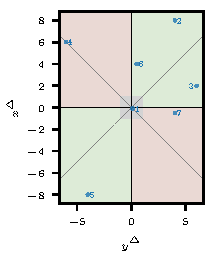
\includegraphics{plots/illustrative_examples/4q_excl_box}
\caption{Four-quadrant plot with rectangular exclusion area.}\label{fig:trending_basic_4q_excl_box}
\end{subfigure}\hspace{0.01\textwidth}%
\begin{subfigure}[t]{.24\textwidth}
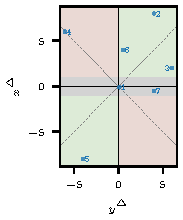
\includegraphics{plots/illustrative_examples/4q_excl_axis}
\caption{Four-quadrant plot with horizontal exclusion area.} \label{fig:trending_basic_4q_excl_axis}
\end{subfigure}\hspace{0.01\textwidth}%
\begin{subfigure}[t]{.24\textwidth}
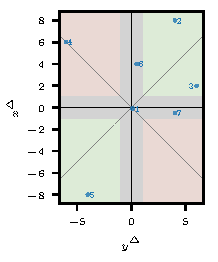
\includegraphics{plots/illustrative_examples/4q_excl_cross}
\caption{Four-quadrant plot with cross-shaped exclusion area.}\label{fig:trending_basic_4q_excl_cross}
\end{subfigure}%
\caption{Illustrations of the four-quadrant plot with sample points and with and without exclusion areas. }
\label{fig:trending_4q}
\end{figure}

\subsection{Trending ratio and other measures}\label{subsec:trending-measures}

Analyzing the number of points in the green versus red quadrants is a standard approach in the trending assessment of measurement data \parencite{Critchley2010,Saugel2015}. 
It boils down to assessing the probability of trending $P(\diffxrv \diffyrv > 0)$, where $\diffyrv$ and $\diffxrv$ denote random variables for future incremental changes, respectively.
Note that $z_1 z_2 > 0$ if and only if $\sign(z_1) = \sign(z_2)$ ($z_1, z_2 \in \R \setminus \{ 0 \}$).
The standard estimator for $P(\diffxrv \diffyrv > 0)$ is
\begin{equation}
    \acc (\diffx, \diffy) \coloneqq \frac{\sum_{t \in \mathcal{T}} \ind{\diffxt \diffyt > 0}}{\card{T}}.\label{eq:acc}
\end{equation}
We refer to this estimator as the trending ratio of the prediction and set $\mathcal{T} = \{1, \dots, T-l\}$.
Visually, the measure computes the fraction of points in the upper right or lower left quadrant.
Such a $2 \times 2$ table of counts is called a contingency table.
It is often used in other scientific areas for evaluation, for example, in dichotomous forecasting or as a confusion matrix in classification analysis~\parencites(see, e.g., the introductions in)()[Ch. 4]{James2021}[Ch. 3]{Jolliffe2012}.
There, a wide range of other methods are usually used to analyze further characteristics of contingency tables.
Two simple measures that focus on specific areas of interest are the positive and negative trending ratios $\accp$ and $\accm$, respectively.
They are defined as
\begin{align}
    \accp (\diffx, \diffy) &\coloneqq \frac{\sum_{t \in \mathcal{T}} \ind{\diffxt \diffyt > 0} \ind{\diffxt > 0}}{\sum_{t \in \mathcal{T}} \ind{\diffxt > 0}} \label{eq:accp}\\
    \accm (\diffx, \diffy) &\coloneqq \frac{\sum_{t \in \mathcal{T}} \ind{\diffxt \diffyt > 0} \ind{\diffxt < 0}}{\sum_{t \in \mathcal{T}} \ind{\diffxt < 0}}\label{eq:accm}
\end{align}
In the classification context, these measures are known as positive or negative predictive value and hit rate or detection failure ratio in forecasting.
They give the probability of a correct prediction of the direction of change, given that the signal direction is positive or negative, respectively.
Therefore, they measure the trending ability of the prediction for positive and negative changes separately by cutting the considered data.
In terms of probability, the two measures give estimates of $P(\diffxrv \diffyrv > 0 | \diffxrv > 0)$ and $P(\diffxrv \diffyrv > 0 | \diffxrv < 0)$, respectively.

The use of these estimators could encourage predictors to exploit imbalances in the number of positive and negative changes. 
A large difference in $\sum_{t \in \mathcal{T}} \ind{\diffyt > 0}$ and $\sum_{t \in \mathcal{T}} \ind{\diffyt < 0}$ is unlikely in the trending setting, as $\diffy$ is obtained from differencing time series data. 
However, if the number of positive and negative $\diffy$ differs widely, the use of unbalanced-data-aware measures should be considered.
There are various adapted measures for unbalanced outcomes, for example, Cohen's $\kappa$ \parencite{Cohen1960} or those listed in \textcite[Table 3.3]{Jolliffe2012}.
Cohen's $\kappa$ is usually used to measure inter-rater agreement and takes into account the ratio of occurred agreement and the probability of agreement by chance.
Cohen's $\kappa$ reduces to rescaling the trending ratio in the case of a $2\times2$-table and balanced outcomes.

All measures can also be evaluated as a rolling estimate to detect changes in performance over time.
A rolling estimate is a sequence of estimates, each computed on a length-$w$-window of the data.
For the trending ratio, a rolling estimate with a backward-looking window is given by
\begin{equation*}
    \acc_t (\diffx, \diffy) \coloneqq \frac{\sum_{t^\star = t-w + 1}^{t} \ind{\diffxt[t^\star] \diffyt[t^\star] > 0}}{w}, \quad t = w-1, \dots, T.\label{eq:acc_rolling}
\end{equation*}
Figure~\ref{fig:trending_ratio_time_series} depicts a rolling window estimate of the trending ratio for the simulated data of Figures~\ref{fig:trending_basic_4q_sample} and~\ref{fig:trending_basic_4q_sample_color}.
Thus, the yearly course of the prediction trending ratio can be detected.
The trending ability of the signal has a strong sinus-shaped seasonality with a trending ability peak after a quarter of a year and a low point after three quarters.
This seasonal behavior cannot be distinguished in the two four-quadrant plots or in the trending ratio.


\begin{figure}
    \centering
    \begin{subfigure}[t]{.24\textwidth}
\includegraphics{plots/illustrative_examples/4Q_sample_without_time}
\caption{Four-quadrant plot with simulated data.}\label{fig:trending_basic_4q_sample}
\end{subfigure}\hspace{0.01\textwidth}
\begin{subfigure}[t]{.24\textwidth}
\includegraphics{plots/illustrative_examples/4Q_sample_with_time}
\caption{The same data is colored according to the time index $t$, the greener, the later.}\label{fig:trending_basic_4q_sample_color}
\end{subfigure}\hspace{0.01\textwidth}
\begin{subfigure}[t]{.48\textwidth}
    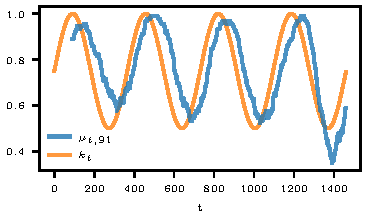
\includegraphics{plots/illustrative_examples/trending_ratio_time_series.pdf}
    \caption{Rolling estimate of the trending ratio over time with window length 91. }\label{fig:trending_ratio_time_series}
    \end{subfigure}%
    \caption{Visualizations for data with a time-varying trending ratio. We defer information on the data generation process in \ref{fig:trending_basic_4q_sample} and \ref{fig:trending_basic_4q_sample_color} to the appendix (see \ref{subsec:app-trending-data-generation}). The trending ratio for the entire data set is $\mu = 0.7577$. The strong seasonality of the trending ratio becomes visible in Figure~\ref{fig:trending_ratio_time_series}. The green curve $k_t$ shows the probability that $\diffxt$ has the same sign as $\diffyt$ for each time step. The rolling estimates are delayed as the windows look backward.}
\end{figure} 

In applications, signal data are often not available for all time steps, for example, due to technical problems or delays in data transfer (see the examples in Sections~\ref{sec:application-covid} and~\ref{sec:application-eda}).
We refer to time steps for which either signal or true values or both are unavailable as missing values.
Pairs of data with missing values can be excluded from the set $\mathcal{T}$ to calculate the measures. 
However, systematical missing values could lead to a biased estimate of the trending ratio, for example, if signal data is omitted in times of high change and thus uncertainty.
In this case, measures should be interpreted with caution, and
inspection of missing data should accompany applications with missing data, for example, through a visual assessment.
In the applications in Sections~\ref{sec:application-covid} and~\ref{sec:application-eda}, only a few missing values occur, and we provide information on the missing data by inspecting the missing data as lists.

\subsection{Accounting for noise and non-informative small changes}\label{subsec:trending-noise}

The above measures use only information on a point's quadrant and neglect further details on its location within the quadrant.
However, points close to the zero point have intuitively less explanatory power or are less reliable.
If there are noise or non-systematic effects present in the true values or predictions, a point's assignment to a quadrant can be driven by noise instead of a systematic trending ability of the signal.
For points with at least one small coordinate, this happens more frequently.

Using an exclusion area around the zero point is a straightforward and highly interpretable extension of the measures of Section~\ref{subsec:trending-measures}.
Points within that area are neither plotted in the four-quadrant plot nor included in the calculation of the measures.
The shape of the exclusion area can be chosen according to the noise characteristics of the predictions and the true values.
In general, it is likely that the prediction models have a noise component and should thus be part of the exclusion area.
We denote the measures of Equations~\eqref{eq:acc},~\eqref{eq:accp} and~\eqref{eq:accm} accounting for an exclusion area $E$ by
\begin{align}
    \acceps (\diffx, \diffy, E) &\coloneqq \frac{\sum_{t \in \mathcal{T}} \ind{\diffx \diffy > 0} \ind{(\diffyt, \diffxt) \notin E}}{\sum_{t \in \mathcal{T}} \ind{(\diffyt, \diffxt) \notin E}}\label{eq:acceps}\\
    \accpeps (\diffx, \diffy, E) &\coloneqq \frac{\sum_{t \in \mathcal{T}} \ind{\diffxt \diffyt > 0} \ind{\diffxt > 0, , (\diffyt, \diffxt) \notin E}}{\sum_{t \in \mathcal{T}} \ind{\diffxt > 0, (\diffyt, \diffxt) \notin E}} \label{eq:accpeps}\\
    \accmeps (\diffx, \diffy, E) &\coloneqq \frac{\sum_{t \in \mathcal{T}} \ind{\diffxt \diffyt > 0} \ind{\diffxt < 0, (\diffyt, \diffxt) \notin E}}{\sum_{t \in \mathcal{T}} \ind{\diffxt < 0, (\diffyt, \diffxt) \notin E}}\label{eq:accmeps}
\end{align}
The measures are then estimators for the probability of trending, given that the change is not in the exclusion area $E$, that is, for $\acceps$, $P(\diffxrv \diffyrv > 0 | \diffxrv \diffyrv \notin E)$.
The estimators accept various shapes of the exclusion area.
Figure~\ref{fig:trending_4q} visualizes different shapes of the exclusion area.
A rectangular exclusion area, $E = \{(x, y) \in \R^2: (-\varepsilon_x \leq x \leq \varepsilon_x) \land (-\varepsilon_y \leq y \leq \varepsilon_y) \}$ 
 ($\varepsilon_x, \varepsilon_y > 0$), leaves out points that are small in both components and, therefore, likely to be driven by noise.
Points where at least the true value or signal is unlikely to be zero are not excluded.
In the example graph in Figure~\ref{fig:trending_basic_4q_excl_box}, only point 1 is excluded.
An exclusion area along one axis, for example, $E = \{(x, y) \in \R^2: (-\varepsilon_x \leq 0 \leq \varepsilon_x)\}$ for $\varepsilon_x > 0$, removes points in which one of the components could change sign by a small amount of noise.
This particularly suits signals where small amounts of noise are inevitable.
A cross-shaped exclusion area, $E = \{(x, y) \in \R^2: (-\varepsilon_x \leq x \leq \varepsilon_x) \lor (-\varepsilon_y \leq y \leq \varepsilon_y) \}$ for $\varepsilon_x, \varepsilon_y > 0$, along both axes accounts for the sign reversal in both components.
For these two methods, points 1 and 7 in Figure~\ref{fig:trending_basic_4q_excl_axis} or 1, 6, and 7 are excluded in Figure~\ref{fig:trending_basic_4q_excl_cross}, respectively.

In addition to these straight shapes, exclusion areas could have more complex shapes, such as ellipses.
Such a shape could, for example, be obtained by using a multivariate normal error model around the zero point and excluding points that exceed a certain likelihood of being produced by chance from the zero point.
These shapes are theoretically appealing, but interpreting the resulting estimators becomes complex.
Thus, we suggest using the above simple exclusion areas.

In most applications, the shape and size of the exclusion area can be chosen based on domain knowledge or expert opinions.
The size estimation can also be based on a proportion of the total variance or the total range of the data.
A third approach is to visualize the trending ratio for different sizes of $E$ and thus inspect the effects of the exclusion area size on the estimates.


\subsection{Bootstrap confidence intervals and the conditional trending plot}\label{subsec:trending-cond-prob}
\unsure{Vielleicht doch zwei subsections?}
Confidence intervals can account for the estimation uncertainty of the measures above.
Bootstrap confidence intervals are a nonparametric technique based on resampling~\parencite[for introductions see][]{Hesterberg2011,Bittmann2021}.
New samples are drawn with replacement from the dataset and are not based on parametric assumptions as classical confidence intervals are.
The confidence interval is then computed based on the bootstrap samples.
We examine three methods for bootstrapping: the intuitive percentile and the more sophisticated basic and \ac{bca} method.
In the \textit{percentile} approach, the confidence interval for the level $\alpha$ is built directly from the empirical distribution of the bootstrap estimators.
The \textit{basic} approach computes the confidence interval based on the non-bootstrap estimate using the bootstrapped quantile deviations~\parencite{Davison1997}.
The \ac{bca} method modifies the quantiles of the empirical bootstrap distribution by a bias and an acceleration parameter~\parencite{Efron1987}.
Typically, the percentile approach needs larger datasets and provides an easy and fast estimate, while the \ac{bca} is computationally expensive but requires smaller datasets for reasonable confidence intervals.
The basic approach balances these two objectives.
We compare the approaches in a small synthetic data study on their small-dataset behavior and computation time in Appendix~\ref{sec:appendix-trending}.
\Ac{bca} is the only method that maintains the confidence level also for small datasets while increasing the computation time only moderately for larger datasets.
Therefore, we use the \ac{bca} method for confidence intervals in the applications in Section~\ref{sec:application}.

The sample is assumed to be independent and identically distributed in standard bootstrapping.
Thus, before applying bootstrapping methods, the strength of sequential dependence should be inspected, for example, by analyzing the autocorrelation and partial autocorrelation.
The simple bootstrapping methods above do not account for serial dependence. 
Bootstrapping focusing on time series data is covered in~\textcite{Hardle2003,Kreiss2012}, for example.

The estimators described above give information on the probabilities $P(\diffxrv \diffyrv > 0 | \diffxrv \diffyrv \notin e)$, $P(\diffxrv \diffyrv > 0 | \diffxrv > 0, \diffxrv \diffyrv \notin e)$ and $P(\diffxrv \diffyrv > 0 | \diffxrv < 0, \diffxrv \diffyrv \notin e)$.
These probabilities draw a general picture but might still be too coarse for local effects.
More insights might be gained by considering the conditional distribution to assess the local trending ability of a prediction.
While it would be possible to build analog measures for other intervals, assessing $P(\diffxrv \diffyrv > 0 | \diffx = x)$ graphically eases the simultaneous evaluation of various intervals.
Furthermore, the graph facilitates the comparison of various methods in a single graph, and asymmetries of $P(\diffxrv \diffyrv > 0 | \diffx = x)$ with respect to $x$ in the trending ability can be detected.
We refer to the plot as a conditional trending plot.

A multivariate \acf{kde} facilitates a continuous estimation of $P(\diffxrv \diffyrv > 0 | \diffxrv = x)$ by estimating the components $f_{\diffxrv, \diffyrv}$ and $f_{\diffxrv}$ of
\begin{align*}
P(\diffxrv \diffyrv > 0 | \diffxrv = x) = \begin{cases}
                                              \int_{-\infty}^0 \frac{f_{\diffxrv, \diffyrv}(x, y)}{f_{\diffxrv}(x)} \ \textrm{d} \: y & \text{if } x < 0, \\
                                              \int_{0}^{\infty} \frac{f_{\diffxrv, \diffyrv}(x, y)}{f_{\diffxrv}(x)} \ \textrm{d} \: y & \text{if } x > 0, \\
\end{cases}
\end{align*}
for $x \neq 0$ through a \ac{kde}.

A comprehensive introduction to multivariate \ac{kde} can be found in \textcite{Gramacki2018}, and implementations are available in many programming languages~\parencite[e.g., for  Python in][]{Seabold2010}.
The \ac{kde} yields estimates for $P(\diffxrv \diffyrv > 0 | \diffxrv = x)$ for all values of $x \in \R$.
Multivariate \ac{kde} takes as modeling parameters a kernel and a bandwidth selector. 
The kernel is usually Gaussian, and there are multiple methods for selecting the bandwidth, each with its own advantages and disadvantages.
Note that for kernels with infinite support, for example, the Gaussian kernel, the plot should be limited to the core values of $\diffx$ without outliers to avoid estimates based on small subsets of the data.

Figure~\ref{fig:trending-cond-prob-bw} shows the resulting conditional trending plots for the three well-known selectors, rule-of-thumb, cross-validation maximum likelihood, and cross-validation least squares using the \verb|statsmodels| Python package~\parencite{Seabold2010}.
While the rule-of-thumb is based only on the covariance matrix, the other two numerically optimize the bandwidth with a hold-one-out least squares or likelihood objective function.
The dashed line shows the theoretical $P(\diffyrv \diffxrv > 0 | \diffxrv = x)$.
The second method, cross-validation least squares, requires long computation times while yielding small or no bandwidth results, even for two relatively small datasets.
The rule-of-thumb and cross-validation maximum likelihood methods yield reasonable results at moderate computation times. 
Further examples, including comparisons between methods regarding their trending ability, are available in Section~\ref{sec:application}.

\begin{figure}
    \centering
    \begin{subfigure}{.48\textwidth}
        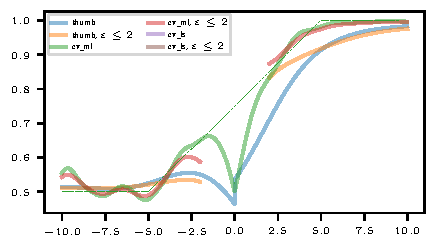
\includegraphics{plots/illustrative_examples/cond_prob_plot_bw_asym_butterfly}
        \caption{First dataset with asymmetric dependence.}
    \end{subfigure}
    \begin{subfigure}{.48\textwidth}
        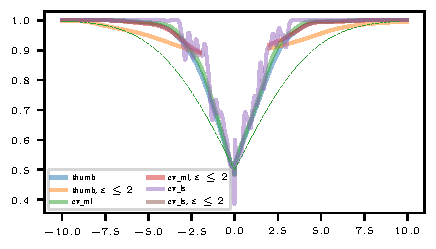
\includegraphics{plots/illustrative_examples/cond_prob_plot_bw_normal}
        \caption{Second dataset. }
    \end{subfigure}
    \caption{Resulting conditional trending plot for different bandwidth selection processes. Cross-validation least squares takes a considerably larger computation time. It does not converge for the first data set and yields a bandwidth too small for the second data set. The rule of thumb is the fastest method but tends to oversmooth. The cross-validation maximum likelihood method yields a more reasonable bandwidth with moderate computation time. }\label{fig:trending-cond-prob-bw}
\end{figure}

\newpage
\subsection{Probabilistic Evaluation}\label{subsec:probabilistic}

In nowcasting and forecasting, there is a shift from point predictions to probabilistic predictions (see, for example, Sections~\ref{sec:application-covid} and~\ref{sec:application-eda} or the review in~\cite{Gneiting2014}).
Probabilistic predictions include a point estimate and information on the forecast uncertainty and quantiles simultaneously.
In this section, we extend the trending assessment to probabilistic predictions.

Probabilistic predictions can take the form of a \ac{cdf}, \ac{pdf}, or quantiles.
The \ac{cdf} is the most general and can be used to derive the others, given they exist.
Let us first assume that the prediction is a \ac{cdf} and the lag is large enough such that the true value is known when issuing the forecast or nowcast.
See the end of the section for predictions given as quantiles or for unknown true values.

Let $F_{t | \tau} (x)$ denote the predicted \ac{cdf} of forecast time $t$ and issue time $\tau$, where the index is analogous to the point prediction notation of Section~\ref{subsec:notation}.
For trending assessment, we compare the probability of positive change with the occurrence of positive changes. 
The probability $p_t$ of a positive change is given by one minus the \ac{cdf} of the prediction at the true value. \unsure{Andere Formulierung für: one minus?}
\unsure{vielleicht sowas: The probability $p_t$ of a positive change is given by the probability that the predicted value at the forecasting time is greater than the known value at the issure time. }
As for the differences in Section~\ref{subsec:notation}, the computation differs slightly for nowcasts and forecasts.
For nowcasts, the probability is calculated by
\begin{equation*}
    p_t = 1 - F_{t+l | t+l} (y_{t})\quad t = 1, \dots, T-l;
\end{equation*}
while for forecasts, it is given by
\begin{equation*}
    p_t = 1 - F_{t+l | t} (y_{t})\quad t = 1, \dots, T-l.
\end{equation*}
Let $z_t$ denote the indicator that the observed change at time $t$ is positive, that is,
\begin{equation*}
    z_t = \ind{\diffyt > 0} \quad t = 1, \dots, T-l.
\end{equation*}
The probabilistic trending evaluation is then based on the probabilities $\mathbf{p} = (p_t)_{t=1}^{T-l}$ and the observed changes $\mathbf{z} = (z_t)_{t=1}^{T-l}$.
The predictive power of $\mathbf{p}$ for $\mathbf{z}$ can be assessed using probabilistic dichotomous forecast evaluation methods.
Dichotomous forecasts predict a binary outcome, for example, a positive or negative change.
Numerical measures for forecast quality are scoring rules.
\unsure{wenn ich hier richtig verstehe, macht man hier quasi aus probabilitsicher Vorhersage zu y eine probabilistische Vorhersage dazu, wie wahrscheinlich die Veränderung positiv ist und dann bewerten. Kann man auch hier auch direkt das dem Bewertungsergbnis schießen, wie gut die Vorhersage auf negative Änderung ist? Wenn ja, vielleicht irgendwie erwähnen oder angeben. }
The \ac{bs} is a widely used scoring rule for dichotomous probabilistic forecasts~\parencite{Brier1950}.
It is defined as
\begin{equation*}
    BS (\mathbf{p}, \mathbf{z}) = \frac{1}{T-l} \sum_{t=1}^{T-l} (p_t - z_t)^2.
\end{equation*}
The \ac{bs} assesses the calibration and sharpness of the forecast and the observation simultaneously~\parencite{Ranjan2010,Mitchell2011}.
Calibration refers to the statistical consistency of forecasts and observations, while sharpness measures the spread of the forecast distribution.
A smaller spread, and thus, higher sharpness, is preferable, as it indicates greater confidence in the prediction.
The basic paradigm of probabilistic forecasting is to maximize sharpness, subject to calibration~\parencite{Gneiting2014}.
These two conflicting aspects cannot be distinguished in the scoring rule.

Graphical models are a standard tool for evaluating solely the calibration of probabilistic forecasts.
In dichotomous forecasting, the reliability diagram is frequently used~\parencite{Ranjan2010}.
The reliability diagram plots the observed frequency of the positive outcome against the predicted probability.
Ideally, the predicted probability equals the observed frequency, and the reliability diagram is a 45-degree line.
Local deviations from the 45-degree line indicate a miscalibration of the forecast for specific probabilities.
Thus, the reliability visualizes the local and overall calibration simultaneously.
For an example of a reliability diagram, see Section~\ref{sec:application-eda}.

If forecasts or nowcasts are given as quantiles, $p_t$ can be determined by interpolations among the quantiles.
Let $q_p$ denote the quantiles for forecast time $t+l$ for even-spaced probabilities $p \in \{1/\pmax, \dots, (p-1) / \pmax\}$ ($\pmax \in \N \setminus \{1, 2\}$) and $y_t$ the true value at time $t$. \unsure{ist das richtig?}
The quantiles $q_p$ generally differ for each time step, but we omit an index here for ease of notation.
The probability $\pc_t$ of a \textit{negative} change is between $p^{\star}$ and $p^{\star} + 1/\pmax$ for
\begin{equation*}
    p^{\star} = \max \{p \in \{1/\pmax, \dots, (\pmax-1) / \pmax\}: q_p \leq y_t\} , \quad \text{if}\ q_{1/\pmax} \leq y_t \leq q_{1 - 1/\pmax}.
\end{equation*}
Quantiles do not determine the location within the interval $[p^{\star}, p^{\star} + 1/\pmax]$.
Under the assumption of a uniform distribution within the quantile interval, the probability of a negative change is
\begin{equation*}
    \bar{p}_t = \frac{y_t - q_{p^\star}}{\pmax (q_{p^{\star} + 1} - q_{p^{\star}})} + p^{\star}.
\end{equation*}
The approach does not assign probabilities for $y_t$ smaller than the smallest quantile $q_{1/p}$ or larger than the largest quantile.
As a simple extension, we assume that the probability mass is uniformly distributed on an interval of the same length as the nearest interval specified by the quantiles.
This yields
\begin{equation*}
\bar{p}_t = \begin{cases}
    \max \{\frac{1}{\pmax} - \frac{q_{p^\star} - y_t}{\pmax (q_{p2/\pmax} - q_{1/\pmax})}, 0\} &, \text{if } y_t < q_{1/p}, \\
    \min \{\frac{1}{\pmax} - \frac{y_t - q_{(\pmax-1)/\pmax}}{\pmax (q_{(\pmax-1)/\pmax} - q_{(\pmax-2)/\pmax})}, 1\} &, \text{if } y_t > q_{1 - 1/p}, \\
    \frac{y_t - q_{p^\star}}{\pmax (q_{p^{\star} + 1} - q_{p^{\star}})} + p^{\star} &, \text{otherwise.}
\end{cases}
\end{equation*}
The probability of positive change is $p_t = 1 - \bar{p}_t$.

If the true value is given as a distribution because it is still unknown, the probabilities $p_t$ can be computed by integration.
Let for two nowcasts the distributions be given by \acp{pdf} $f_{t+l|t+l}$ and $f_{t|t+l}$ with \acp{cdf}  $F_{t+l|t+l}$ and $F_{t|t+l}$.
Then, the probability of a negative change can be computed by
\begin{align}
    \bar{p}_t
        &= \int_{\begin{subarray}{l}x_1, x_2 \in \R: \\ x_2 < x_1\end{subarray}} f_{t|t+l} (x_1) f_{t+l|t+l} (x_2)  \ \textrm{d} \: x_2 \ \textrm{d} \: x_1 \nonumber\\
        &= \int_{x_1 \in \R} \int_{-\infty}^{x_1} f_{t|t+l} (x_1) f_{t+l|t+l} (x_2)  \ \textrm{d} \: x_2 \ \textrm{d} \: x_1 \nonumber\\
        &= \int_{x_1 \in \R} f_{t|t+l} (x_1) F_{t+l|t+l} (x_1)  \ \textrm{d} \: x_2 \ \textrm{d} \: x_1 \label{eq:trending-probabilistic-pdf}.
\end{align} \unsure{vielleicht eher d(x,y) wegen einem Integralzeichen?}

\unsure{Die Unabhängigkeitsannahme ist nicht zu streng? weil es ist ja eigentlich die Aufgabe von einenm guten Nowcaster diese Abhängigkeit zu modellieren oder?}
Thereby, the distributions are assumed to be independent.
As a Monte Carlo approximation of Equation~\eqref{eq:trending-probabilistic-pdf}, the probability can also be calculated by sampling from $f_{t+l|t+l}$ and $f_{t|t+l}$ and calculating the fraction of negative changes.
For forecasts, the indexes have to be shifted.
If no \acp{pdf} are available, they can be estimated from the \ac{cdf} or quantiles, or the \ac{cdf} or quantiles can be used to generate samples for the Monte Carlo approximation.


%\section{Simulation Studies (?)}
%
%Eher nicht, weil angewandtes Paper

\section{Application to real-world data} \label{sec:application}
In this section, we evalute the trending in three different applications.
In the first application in Section~\ref{sec:application-covid}, we consider the nowcasting of the seven-day hospitalization rate for COVID-19 in Germany.
Section~\ref{sec:application-eda} applies the trending assessment to forecast methods for the number of arrivals in a large emergency department.
In the last application in Section~\ref{sec:application_measurement}, we consider the trending assessment of non-invasive blood pressure measurements compared to invasive blood pressure measurements.

\subsection{Covid nowcasting} \label{sec:application-covid}

Amid the COVID-19 pandemic, the importance of accurate and prompt nowcasts of the pandemic's progression has become evident.
Various indicators measured the pandemic's spread and severity. 
In Germany, the seven-day hospitalization rate was established as a central steering measure for COVID-19 measures in November 2021, and the imposition of severe public restrictions was based on it~\citep{RobertKochInstitute2021}. 
The Robert Koch Institute (RKI) provided preliminary daily reports on the seven-day hospitalization rate.
However, these reports were subject to severe delays and revisions in two sources.
The first source is technical delays in the reporting process, for example, due to different authorities passing the data to the RKI~\citep{RobertKochInstitute2024}.
The second, more systematic source is the structure of the seven-day hospitalization rate.
To a given date, all the cases are allocated whose first positive test result was on that date and who were hospitalized in relation to the disease in the following.
The seven-day hospitalization rate is the average number of those cases per $100,000$ inhabitants on the given date and six days before.
Thus, the final seven-day hospitalization rate can only be reported with a significant delay of more than 70 days, as the hospitalization of infected inhabitants can occur much later than the first positive test.
Nevertheless, as the seven-day hospitalization rate was considered a major indicator of the pandemic's development, many organizations and institutions started to issue nowcasts, including research teams and newspapers.
To collect nowcasts of the seven-day hospitalization rate by different nowcast groups, the COVID19-Nowcasting-Hub was established~\citep{ChairOfEconometricsAndStatisticsAtKarlsruheInstituteOfTechnology2024}.
The nowcasts contain the seven-day hospitalization rate's predictive mean, median, and other quantiles.

\begin{figure}
    \centering
    \begin{subfigure}[t]{0.48\textwidth}
    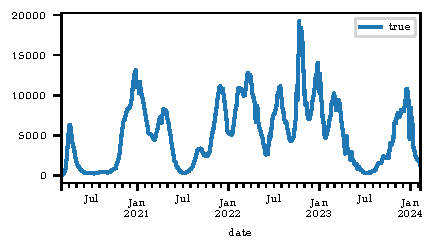
\includegraphics{plots/covid_nowcast/00_true_data.pdf}
    \caption{Realisations.}
    \label{fig:app-covid-true}
    \end{subfigure}\hfill
    \begin{subfigure}[t]{0.48\textwidth}
    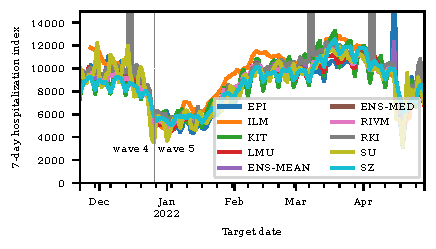
\includegraphics{plots/covid_nowcast/00_nowcast_data.pdf}
    \caption{Same-day nowcasts.}
    \label{fig:app-covid-nowcast}
        \end{subfigure}
    \caption{True and nowcast data of the seven-day-hospitalization in Germany from November 22, 2021, to April 29, 2022 \citep{ChairOfEconometricsAndStatisticsAtKarlsruheInstituteOfTechnology2024}.
    The outliers in the RKI model of values above $10^8$ are removed before the following analysis.}
    \label{fig:app-covid-true-nowcast}
\end{figure}

The data contains eight nowcasts from scientific and public institutions, nowcast communities, and a newspaper, using different input variables, calendar data, and length of training data.
The model structures are diverse, including Bayesian models, generalized additive models, and parametric bootstrapping.
Table~\ref{tab:app-covid-models} in the appendix lists the different abbreviations and the respective names in the COVID19-Nowcasting-Hub.
For information on the model design, we refer to~\citet{Wolffram2023}.
Using the nowcasts, two ensemble methods are constructed using the ensembles' mean or median.
We denote them by ENS-MEAN and ENS-MED.
\citet{Wolffram2023} describes the design of the nowcast tasks and the data submission guidelines for the teams stated in a preregistered study. 
In line with the initial study design, we consider the period from November 22, 2021, to April 29, 2022, as the evaluation period.
For the true values, we use the data from February 8, 2024.
The nowcasts are resolved with regard to all inhabitants and specific geographical and age breakdowns.
We do not expand on the models' performance on specific regions or age groups in Germany and the probabilistic nowcast assessment.
Figure~\ref{fig:app-covid-true-nowcast} displays the true and nowcast data for the evaluation period.
The time comprises the fourth wave's end in December 2021 and nearly the entire fifth wave of the pandemic in Germany, lasting until May 28, 2022~\citep{Tolksdorf2022}.

Table~\ref{tab:app-covid-rmse} summarizes the point evaluation measures for the issued mean of the different models.
The models issue same-day nowcasts for nearly all 159 days of the evaluation period~\citep[for explanations of the missing values, see][Tables A2, A3, and A4]{Wolffram2023}.
The best-performing models in terms of RMSE and MAE are the ILM and RKI models.
The ensemble methods perform worse than the best models regarding the mean location.
The performance of the models is diverse, with more than twice as high RMSE values for the worst models compared to the best models.
Note that the high values for the EPI model could be driven by an exceptionally far-off value at the end of the evaluation period.

In addition to close inspection of the point evaluation measures, assessing the trending of the nowcasts is crucial.
To assess the impact of taken measures and the direction of the curve, it is essential to distinguish between rising and falling hospitalization rates.
If hospitalization rates rise, measures should be tightened, while falling rates might allow for loosening measures.
Especially, asymmetries are of interest to assess whether some models are better at recognizing a fall than a rise or vice versa.

\begin{table}[]
    \centering
    \begin{tabular}{llllr}
\toprule
 & rmse & mae & mse & count \\
model &  &  &  &  \\
\midrule
ILM-prop & :,.f & :,.f & :,.f & 530 \\
RIVM-KEW & :,.f & :,.f & :,.f & 817 \\
NowcastHub-MeanEnsemble & :,.f & :,.f & :,.f & 610 \\
NowcastHub-MedianEnsemble & :,.f & :,.f & :,.f & 610 \\
LMU_StaBLab-GAM_nowcast & :,.f & :,.f & :,.f & 574 \\
RKI-weekly_report & :,.f & :,.f & :,.f & 334 \\
KIT-simple_nowcast & :,.f & :,.f & :,.f & 861 \\
SZ-hosp_nowcast & :,.f & :,.f & :,.f & 535 \\
SU-hier_bayes & :,.f & :,.f & :,.f & 423 \\
Epiforecasts-independent & :,.f & :,.f & :,.f & 275 \\
\bottomrule
\end{tabular}

    \caption{Point evaluation measures for the issued mean of the different models. The evaluation period comprises 159 days. }
    \label{tab:app-covid-rmse}
\end{table}

\subsubsection*{Results}

In the following, we apply the trending assessment of Section~\ref{sec:trending} to the nowcasts of the seven-day hospitalization rate.
We report the trending for the horizons 1, 7, and 14 days.
While horizon one assesses the short-term trending, horizons seven and 14 consider the medium-term trending.
The horizons seven and 14 are particularly interesting, reflecting a usual period until new policy changes are taken.

Before stating the results, we provide background information on the marginal distributions of the true values and nowcasts for the different horizons.
Table~\ref{tab:app-covid-marginals} in Appendix~\ref{sec:appendix-application-covid} presents marginal statistics such as standard deviation and quantiles of the nowcasts and true values.
Overall, the variability and general level of differences grow with the horizon.
The standard deviation increases from roughly 300 for horizon one to 1,200 for horizon seven and 2,000 for horizon 14 days.
Similarly, the 10\%-quantile of differences increases.
The 10\%-quantile is used for the exclusion areas in the trending assessment.
The exclusion area is rectangular; a point falls within it if both $\diffy$ and $\diffx$ are below the respective 10\%-quantile of the absolute differences.
Thus, points are still included in the trending assessment if they are large in one dimension but not in the other, thus ensuring that substantial changes in, for example, $\diffy$ are to be recognized by the nowcast and vice versa.

Table~\ref{tab:app-covid-trending-ratios-lag-7} lists the trending ratios for all models with and without exclusion areas for the horizon of seven days.
The trending ratios without exclusion area range from 0.72 to 0.85 for the horizon of seven days.
The negative trending ratios are higher than the positive trending ratios for all models.
The confidence intervals for the positive and negative trending ratios do not overlap for all models, indicating that the trending ratios are indeed different.
The 10\%-quantile exclusion areas have, at most, an influence of 0.03 on the ratios.
The model with the highest trending ratio is the ILM model, and the model with the lowest is the RKI model.
The confidence intervals between all models overlap.
The positive trending ratio implies a similar ranking of the models, while the negative ratio is second best for the RKI model.
For the horizons of one and 14 days, we refer to Table~\ref{tab:app-covid-trending-ratios-lag-1-14} in Appendix~\ref{sec:appendix-application-covid}.

Figure~\ref{fig:app-covid-cond-prob-trending-ratio-7} shows the conditional trending plots and the trending ratio over the exclusion area for the horizon seven days; the respective plots for the horizons one day and 14 days are shown in Figure~\ref{fig:app-covid-cond-prob-trending-ratio-1-14}.
Here, only the best models in point evaluation measures, ILM, RKI, RIVM, and ENS-MED, are shown to keep the plots easily readable.
If RKI or ILM issues a fall in the hospitalization rate, the probability of a fall is higher than if RIVM or ENS-MED issues a fall.
The opposite is the case for a nowcasted hospitalization rate increase, and the difference between the models' performance is higher.
Similar observations can be made for the horizon of 14 days in Figure~\ref{fig:app-covid-cond-prob-14}.
For a horizon of one day, the models' conditional trending ability difference is less pronounced (see Figure~\ref{fig:app-covid-cond-prob-1}).
The RKI model is still less conclusive when issuing an increase in the hospitalization rate, while RIVM is most informative in that case.
The curves cross for an issued fall, with ENS-MED being on top for issued falls above 250.

The trending ratios for various exclusion areas are shown in Figure~\ref{fig:app-covid-trending-ratio-7}.
In general, the trending ratio increases with larger exclusion areas.
While the RIVM and ENS-MED trending ratios evolve similarly, the RKI and ILM trending ratios get closer.
For the horizon of one day, the RKI trending ratio decreases with increasing exclusion area size while the other models rise (see Figure~\ref{fig:app-covid-trending-ratio-1}).
For the horizon of 14 days, all trending ratio curves increase with the exclusion area size (see Figure~\ref{fig:app-covid-trending-ratio-14}).

\begin{table}
    \centering
    \tiny
    \begin{tabular}{l p{0.11\textwidth} p{0.11\textwidth} p{0.11\textwidth} p{0.11\textwidth} p{0.11\textwidth} p{0.11\textwidth}}
\toprule
 & $\mu^{7}$ & $\mu^{+, 7}$ & $\mu^{-, 7}$ & $\mu^{7}_{q_{0.1}}$ & $\mu^{+, 7}_{q_{0.1}}$ & $\mu^{-, 7}_{q_{0.1}}$ \\
\midrule
EPI & {0.77\newline(0.71, 0.82)} & {0.67\newline(0.59, 0.76)} & {0.87\newline(0.79, 0.92)} & {0.78\newline(0.72, 0.83)} & {0.68\newline(0.59, 0.75)} & {0.88\newline(0.80, 0.93)} \\
ILM & {0.85\newline(0.80, 0.90)} & {0.73\newline(0.64, 0.80)} & {0.99\newline(0.94, 1.00)} & {0.85\newline(0.80, 0.90)} & {0.74\newline(0.65, 0.81)} & {0.99\newline(0.94, 1.00)} \\
KIT & {0.74\newline(0.68, 0.80)} & {0.64\newline(0.55, 0.72)} & {0.87\newline(0.80, 0.93)} & {0.75\newline(0.69, 0.80)} & {0.64\newline(0.55, 0.72)} & {0.88\newline(0.81, 0.94)} \\
LMU & {0.80\newline(0.74, 0.85)} & {0.70\newline(0.62, 0.77)} & {0.91\newline(0.84, 0.95)} & {0.81\newline(0.75, 0.86)} & {0.72\newline(0.63, 0.79)} & {0.92\newline(0.85, 0.96)} \\
ENS-MEAN & {0.82\newline(0.76, 0.86)} & {0.71\newline(0.63, 0.78)} & {0.94\newline(0.89, 0.97)} & {0.82\newline(0.76, 0.87)} & {0.71\newline(0.63, 0.78)} & {0.96\newline(0.90, 0.99)} \\
ENS-MED & {0.82\newline(0.77, 0.86)} & {0.70\newline(0.61, 0.78)} & {0.96\newline(0.90, 0.99)} & {0.83\newline(0.77, 0.87)} & {0.72\newline(0.64, 0.79)} & {0.96\newline(0.90, 0.99)} \\
RIVM & {0.83\newline(0.77, 0.87)} & {0.74\newline(0.65, 0.81)} & {0.92\newline(0.86, 0.96)} & {0.83\newline(0.78, 0.88)} & {0.74\newline(0.65, 0.81)} & {0.93\newline(0.87, 0.97)} \\
RKI & {0.72\newline(0.65, 0.77)} & {0.60\newline(0.51, 0.67)} & {0.98\newline(0.92, 1.00)} & {0.73\newline(0.66, 0.78)} & {0.61\newline(0.53, 0.68)} & {0.98\newline(0.92, 1.00)} \\
SU & {0.81\newline(0.75, 0.86)} & {0.71\newline(0.62, 0.79)} & {0.92\newline(0.85, 0.96)} & {0.81\newline(0.75, 0.85)} & {0.71\newline(0.63, 0.79)} & {0.92\newline(0.85, 0.96)} \\
SZ & {0.78\newline(0.72, 0.83)} & {0.67\newline(0.58, 0.75)} & {0.91\newline(0.84, 0.96)} & {0.78\newline(0.72, 0.83)} & {0.67\newline(0.58, 0.75)} & {0.92\newline(0.85, 0.97)} \\
\bottomrule
\end{tabular}

    \caption{The trending ratio $\accl[7]$, positive trending ratio $\accpl[7]$, and negative trending ratio $\accml[7]$ for the models with and without exclusion areas for the horizon seven days. The exclusion areas are rectangles centered on the zero points with a width and height of twice the 10\%-quantile of the absolute values of nowcast and true values. }
    \label{tab:app-covid-trending-ratios-lag-7}
\end{table}

\begin{figure}
    \centering
%    \includegraphics{}
    \begin{subfigure}[t]{.48\textwidth}
    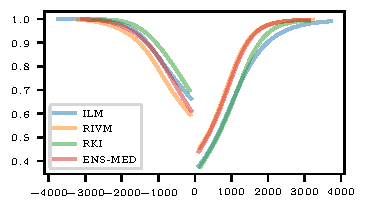
\includegraphics{plots/covid_nowcast/40_cond_prob_lag_7}
    \caption{Conditional trending plot.}\label{fig:app-covid-cond-prob-7}
    \end{subfigure}\hfill
    \begin{subfigure}[t]{.48\textwidth}
    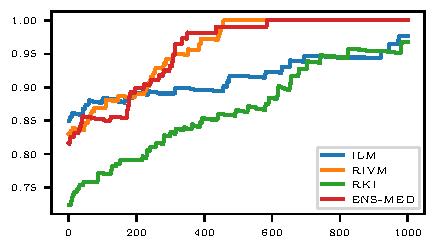
\includegraphics{plots/covid_nowcast/40_acc_eps_lag_7}
    \caption{Trending ratio over exclusion area size in $\diffx$.}\label{fig:app-covid-trending-ratio-7}
    \end{subfigure}
    \caption{Conditional trending plot and trending ratio over exclusion area for the nowcasts of the seven-day hospitalization rate ILM, RKI, RIVM, and ENS-MED for the horizon seven days.}
    \label{fig:app-covid-cond-prob-trending-ratio-7}
\end{figure}



\subsubsection*{Discussion}

For all horizons, the influence of the exclusion area on the 10\%-quantile level is negligible.
For example, the trending ratio changes at most by 0.03 for the EPI model with $\accml[14]$.
The exclusion areas are thus not crucial for the trending assessment in the case of the nowcasts of the seven-day hospitalization rate.
The lower bound of confidence intervals is at least 0.68 for all models, indicating that they perform better than random guessing the trend.

Trending assessment evaluates the models differently from point evaluation measures.
RKI is among the best in point evaluation measures but performs worse in trending assessment.
The assessment of asymmetry in the conditional trending plots is crucial for interpreting the trending ratios, with the RKI model being the most prominent example.

Figure~\ref{fig:app-covid-trending-ratio-7} shows that the trending ratio increases with larger exclusion areas. 
This indicates that if the model predicts a large change, the direction is indeed better than when a small change is predicted.

A more extensive training size would be beneficial for assessing the models' performance.
For the evaluation period of 159 days, the trending ratio confidence intervals overlap; thus, no conclusions can be drawn from the trending evaluation.

\subsection{Forecasting emergency department arrivals}\label{sec:application-eda}

In a second example, we consider forecasting the hourly number of arrivals in a large emergency department.
Good forecasts are crucial for planning staff and resources.
Several models are used for predicting hourly outcomes in a study by \citet{Rostami-Tabar2023}.
Every 12 hours, the models issue hourly forecasts for the next 48 hours.
Thus, the management can take measures according to the expected number of arrivals, for example, through redeploying staff and reconfiguring units.

\citet{Rostami-Tabar2023} publish means and probabilistic quantile forecasts, which are evaluated through RMSE, pinball loss, pinball skill scores, and PIT-histograms.
The models are trained on data from April 1, 2014, to February 28, 2018, and evaluated on data from March 1, 2018, to February 28, 2019.
For further notes on the models and the evaluation, we refer to \citet{Rostami-Tabar2023}.
From the issued forecasts, we use the mean as a point forecast for the trending assessment and evaluate the probabilistic trending subsequently.
We use the forecasts issued at the first time point for every target time.
Thus, the forecasts are issued 36 to 48 hours ahead of the target time, and the emergency department management has time to adjust the measures according to the expected number of arrivals.
Considering only the forecasts of at least 36 hours ahead, we restrict the evaluation period to March 2, 2018, at noon, to February 28, 2019, at 23:00, comprising 8,724 hours.

In this setup, trending assessment is a simple and intuitive way to assess the models' performance.
The trending perspective is easy for the management to understand and implement, as simple comparisons of the expected workload to a recent shift can be made.
If, for example, the staff was near capacity in the last shift and an increase in the number of arrivals is expected, the management can take measures to adjust the workload.

The number of arrivals has a strong weekly and daily pattern.
Thus, we consider the horizons of 72 hours, the last already observed shift of the same hour of day, and seven days, the previous shift of the same hour and day.
Table~\ref{tab:app-eda-point-evaluation} lists the point evaluation measures and the count of available forecasts.
The best-performing models regarding RMSE and MAE are the NBI-2 and Poisson-2 models.
More than 8,600 forecasts are available for all models, with differences in the number due to missing values on four afternoons in 2018.
Note that the reported values for the RMSE differ from those in \citet{Rostami-Tabar2023}.
In contrast to their work, we use only the forecast data at least 36 hours ahead and not the entire forecast data for evaluation.

\begin{table}
\centering
\begin{tabular}{l r r r}
\toprule
Model & RMSE & MAE & Count \\
\midrule
NBI-2 & 8.883 & 3.200 & 8688 \\
Poisson-2 & 8.884 & 3.200 & 8688 \\
Poisson-1 & 9.164 & 3.238 & 8688 \\
Benchmark-2 & 9.246 & 3.236 & 8688 \\
Ttr-2 & 9.394 & 3.266 & 8688 \\
NOtr-1 & 9.413 & 3.276 & 8688 \\
NOtr-2 & 9.413 & 3.276 & 8688 \\
Poisson-2-I & 9.458 & 3.276 & 8688 \\
Benchmark-1 & 10.065 & 3.331 & 8688 \\
GBM-2 & 11.663 & 3.542 & 8688 \\
tbats & 12.905 & 3.912 & 8724 \\
Prophet & 13.078 & 3.877 & 8724 \\
qreg-1 & 13.337 & 3.758 & 8688 \\
Regression-Poisson & 21.162 & 4.818 & 8724 \\
ADAM-iETSX & 28.000 & 5.561 & 8724 \\
ETS & 29.358 & 5.742 & 8724 \\
\bottomrule
\end{tabular}

\caption{Point evaluation measures for the models. The smaller count for some models stems from missing forecasts scattered throughout the evaluation period.}\label{tab:app-eda-point-evaluation}
\end{table}


\subsubsection*{Results}

Table~\ref{tab:app-eda-marginals} analyzes the differences in marginal distributions for the forecasts and true values for the horizons of three and seven days.
Note that the difference definition aligns with Section~\ref{subsec:notation}, defined as the difference between the forecasted mean and true value of three and seven days before, as the true value is available when issuing the forecast.
The fraction of positive differences varies between 0.39 and 0.63 for the horizon of three days and between 0.37 and 0.63 for the horizon of seven days.
The variability of differences decreases for the larger horizon for most models; only for the ETS model does it increase.
The 10\%-quantile of the differences is between zero and one for all models and horizons.
Thus, we exclude only differences smaller than one from the trending assessment.
The resulting fraction of included values in the computation is also listed in Table~\ref{tab:app-eda-marginals} and is at least 79\% of the values.

\begin{table}
    \centering
    \tiny
    \begin{tabular}{lllllllll}
\toprule
 & (1), l=3 & $\sigma_{x^{\Delta, 3}}$ & $q_{0.1} (x^{\Delta, 3})$ & (2), l=3 & (1), l=7 & $\sigma_{x^{\Delta, 7}}$ & $q_{0.1} (x^{\Delta, 7})$ & (2), l=7 \\
\midrule
ADAM-iETSX & 0.57 & 7.76 & 0.83 & 0.88 & 0.57 & 7.49 & 0.78 & 0.87 \\
Benchmark-1 & 0.45 & 5.05 & 0.50 & 0.80 & 0.44 & 4.43 & 0.47 & 0.78 \\
Benchmark-2 & 0.51 & 5.11 & 0.52 & 0.80 & 0.50 & 4.29 & 0.45 & 0.78 \\
ETS & 0.58 & 7.49 & 0.78 & 0.87 & 0.58 & 7.68 & 0.84 & 0.88 \\
GBM-2 & 0.39 & 4.93 & 0.51 & 0.80 & 0.37 & 4.61 & 0.49 & 0.79 \\
NBI-2 & 0.53 & 5.04 & 0.52 & 0.81 & 0.53 & 4.41 & 0.48 & 0.79 \\
NOtr-1 & 0.52 & 5.03 & 0.51 & 0.81 & 0.51 & 4.41 & 0.49 & 0.79 \\
NOtr-2 & 0.52 & 5.03 & 0.51 & 0.81 & 0.51 & 4.41 & 0.49 & 0.79 \\
Poisson-1 & 0.53 & 5.04 & 0.51 & 0.81 & 0.52 & 4.38 & 0.48 & 0.79 \\
Poisson-2 & 0.53 & 5.05 & 0.52 & 0.80 & 0.53 & 4.42 & 0.48 & 0.78 \\
Poisson-2-I & 0.51 & 5.03 & 0.51 & 0.81 & 0.50 & 4.42 & 0.49 & 0.79 \\
Prophet & 0.62 & 5.27 & 1.00 & 0.91 & 0.62 & 5.15 & 1.00 & 0.91 \\
Regression-Poisson & 0.51 & 6.65 & 0.67 & 0.85 & 0.51 & 6.49 & 0.67 & 0.85 \\
Ttr-2 & 0.51 & 5.03 & 0.50 & 0.81 & 0.50 & 4.41 & 0.49 & 0.79 \\
qreg-1 & 0.39 & 5.01 & 0.49 & 0.81 & 0.39 & 4.84 & 0.51 & 0.80 \\
tbats & 0.63 & 5.35 & 1.00 & 0.92 & 0.63 & 5.04 & 1.00 & 0.92 \\
True & 0.54 & 6.61 & 1.00 & 0.93 & 0.55 & 5.90 & 1.00 & 0.92 \\
\bottomrule
\end{tabular}

    \caption{Marginal analysis of the nowcast and true differences. The column (1) shows the fraction of values greater than zero for horizon $l$, $\sigma_{x^{\Delta, l}}$ the standard deviation, and $q_{0.1} (x^{\Delta, l})$ the 10\% quantile of the differences' absolute values.}
    \label{tab:app-eda-marginals}
\end{table}

Table~\ref{tab:app-eda-trending-ratios} lists the trending ratios for all models for three and seven-day horizons.
The trending ratios range from 0.68 to 0.84 for a horizon of three days and from 0.68 to 0.82 for seven days.
The negative and positive trending ratios differ for all models and horizons.
For some models, for example, the GBM-2 model, the positive trending ratio is higher; for some models, for example, the tbats model, the negative trending ratio is higher.
The confidence interval width is at most 0.02 for the trending ratios and at most 0.03 for the positive and negative trending ratios.
The models GBM-2, qreg-1, and Benchmark-1 have the highest positive trending ratio for three and seven days horizon, while Poisson-2 and NBI-2 have the highest negative trending ratio.

Figure~\ref{fig:app-eda-cond-prob} shows the conditional trending plots for the models Benchmark-1, GBM-2, NBI-2, Poisson-2, and qreg-1 for the horizons three and seven days and thus inspects the local trending ability of the models with highest positive and negative trending ratio.
The conditional trending plots show similar courses for the two horizons, while the curves are shifted downwards for the horizon of seven days.
The model's relative trending ability evolves consistently for the two horizons, with the NBI-2 and Poisson-2 models being indistinguishable.
The GBM-2 model outperforms the qreg-1 model for all $x$.
The models NBI-2 and Poisson-2 have the highest trending ability for all negative values of $x$ and the lowest trending ability for all positive values of $x$.
Benchmark-1 lies between the other models for all $x$.

Figure~\ref{fig:app-eda-prob} visualizes the probabilistic trending evaluation for the same subset of models.
The \acfp{bs} are shown in Figure~\ref{fig:app-eda-prob-brier}, and the reliability diagrams for the horizons three and seven days are shown in Figures~\ref{fig:app-eda-prob-rel-3} and \ref{fig:app-eda-prob-rel-7}.
The \acp{bs} are smallest for NBI-2 and Poisson-2 for both horizons, while the \acp{bs} for the other models are larger and differ more.
The qreg-1 model has the highest \ac{bs} for both horizons.
The reliability diagrams of GBM-2 and NBI-2 are also close and show a too-small fraction of increases for the predicted probability overall.
For the other models, the reliability diagrams show a fraction of increases that are too large for the corresponding predicted probability.

\begin{table}
    \centering
    \tiny
    \begin{tabularx}{\textwidth}{X p{0.11\textwidth} p{0.11\textwidth} p{0.11\textwidth} p{0.11\textwidth} p{0.11\textwidth} p{0.11\textwidth}}
\toprule
 & $\mu^{3}$ & $\mu^{+, 3}$ & $\mu^{-, 3}$ & $\mu^{7}$ & $\mu^{+, 7}$ & $\mu^{-, 7}$ \\
\midrule
ADAM-iETSX & {0.70\newline(0.69, 0.71)} & {0.68\newline(0.67, 0.69)} & {0.72\newline(0.71, 0.73)} & {0.68\newline(0.67, 0.69)} & {0.67\newline(0.66, 0.69)} & {0.69\newline(0.67, 0.70)} \\
Benchmark-1 & {0.83\newline(0.82, 0.84)} & {0.86\newline(0.85, 0.87)} & {0.81\newline(0.79, 0.82)} & {0.81\newline(0.80, 0.82)} & {0.86\newline(0.85, 0.87)} & {0.78\newline(0.76, 0.79)} \\
Benchmark-2 & {0.84\newline(0.83, 0.84)} & {0.83\newline(0.82, 0.85)} & {0.84\newline(0.83, 0.85)} & {0.82\newline(0.81, 0.83)} & {0.83\newline(0.82, 0.84)} & {0.80\newline(0.79, 0.82)} \\
ETS & {0.68\newline(0.67, 0.69)} & {0.66\newline(0.65, 0.67)} & {0.70\newline(0.69, 0.72)} & {0.67\newline(0.66, 0.68)} & {0.66\newline(0.64, 0.67)} & {0.68\newline(0.66, 0.69)} \\
GBM-2 & {0.82\newline(0.81, 0.82)} & {0.90\newline(0.89, 0.91)} & {0.77\newline(0.76, 0.78)} & {0.78\newline(0.77, 0.79)} & {0.88\newline(0.87, 0.90)} & {0.73\newline(0.72, 0.74)} \\
NBI-2 & {0.84\newline(0.83, 0.85)} & {0.83\newline(0.82, 0.84)} & {0.85\newline(0.84, 0.86)} & {0.82\newline(0.81, 0.83)} & {0.82\newline(0.81, 0.83)} & {0.82\newline(0.81, 0.83)} \\
NOtr-1 & {0.83\newline(0.83, 0.84)} & {0.83\newline(0.82, 0.84)} & {0.84\newline(0.82, 0.85)} & {0.81\newline(0.80, 0.82)} & {0.82\newline(0.81, 0.83)} & {0.80\newline(0.79, 0.81)} \\
NOtr-2 & {0.83\newline(0.83, 0.84)} & {0.83\newline(0.82, 0.84)} & {0.84\newline(0.82, 0.85)} & {0.81\newline(0.80, 0.82)} & {0.82\newline(0.81, 0.83)} & {0.80\newline(0.79, 0.81)} \\
Poisson-1 & {0.84\newline(0.83, 0.84)} & {0.82\newline(0.81, 0.83)} & {0.85\newline(0.84, 0.86)} & {0.82\newline(0.81, 0.82)} & {0.82\newline(0.81, 0.83)} & {0.81\newline(0.80, 0.82)} \\
Poisson-2 & {0.84\newline(0.83, 0.85)} & {0.83\newline(0.82, 0.84)} & {0.85\newline(0.84, 0.86)} & {0.82\newline(0.81, 0.82)} & {0.82\newline(0.81, 0.83)} & {0.82\newline(0.80, 0.83)} \\
Poisson-2-I & {0.83\newline(0.83, 0.84)} & {0.84\newline(0.83, 0.85)} & {0.83\newline(0.82, 0.84)} & {0.81\newline(0.80, 0.82)} & {0.83\newline(0.81, 0.84)} & {0.80\newline(0.79, 0.81)} \\
Prophet & {0.75\newline(0.74, 0.76)} & {0.72\newline(0.71, 0.73)} & {0.79\newline(0.77, 0.80)} & {0.74\newline(0.73, 0.74)} & {0.72\newline(0.70, 0.73)} & {0.76\newline(0.75, 0.77)} \\
Regression-Poisson & {0.72\newline(0.71, 0.73)} & {0.73\newline(0.71, 0.74)} & {0.72\newline(0.70, 0.73)} & {0.70\newline(0.69, 0.71)} & {0.71\newline(0.70, 0.73)} & {0.69\newline(0.67, 0.70)} \\
Ttr-2 & {0.84\newline(0.83, 0.84)} & {0.84\newline(0.83, 0.85)} & {0.83\newline(0.82, 0.85)} & {0.81\newline(0.80, 0.82)} & {0.83\newline(0.82, 0.84)} & {0.80\newline(0.79, 0.81)} \\
qreg-1 & {0.80\newline(0.79, 0.80)} & {0.88\newline(0.87, 0.89)} & {0.75\newline(0.74, 0.76)} & {0.77\newline(0.76, 0.78)} & {0.86\newline(0.85, 0.88)} & {0.71\newline(0.70, 0.72)} \\
tbats & {0.75\newline(0.74, 0.76)} & {0.72\newline(0.71, 0.73)} & {0.80\newline(0.78, 0.81)} & {0.73\newline(0.72, 0.74)} & {0.71\newline(0.69, 0.72)} & {0.76\newline(0.74, 0.77)} \\
\bottomrule
\end{tabularx}

    \caption{Trending ratio $\acc$, positive trending ratio $\accp$, and negative trending ratio $\accm$ for the models with the exclusion of zero-containing points for the horizons 72 hours and seven days.}
    \label{tab:app-eda-trending-ratios}
\end{table}

\begin{figure}
    \centering
    \begin{subfigure}[t]{0.48\textwidth}
    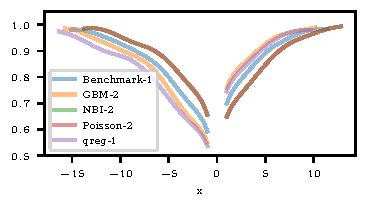
\includegraphics{plots/ed_arrival/50_Cond_Prob_lag_3}
    \caption{Horizon three days}
    \end{subfigure}\hfill
    \begin{subfigure}[t]{0.48\textwidth}
    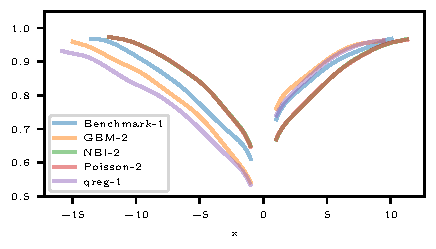
\includegraphics{plots/ed_arrival/50_Cond_Prob_lag_7}
    \caption{Horizon seven days}
    \end{subfigure}
    \caption{Conditional trending plots for the horizons three and seven days and the models with the best positive or negative trending ability. The plots of NBI-2 and Poisson-2 are indistinguishable.}
    \label{fig:app-eda-cond-prob}
\end{figure}

\begin{figure}
    \begin{subfigure}{0.32\textwidth}
    \tiny
    \begin{tabular}{lll}
\toprule
 & 3 d & 7 d \\
\midrule
Benchmark-1 & 0.1586 & 0.1761 \\
GBM-2 & 0.1590 & 0.1759 \\
NBI-2 & 0.1549 & 0.1717 \\
Poisson-2 & 0.1549 & 0.1714 \\
qreg-1 & 0.1679 & 0.1843 \\
\bottomrule
\end{tabular}

    \caption{Brier Scores for the different models and horizons.}\label{fig:app-eda-prob-brier}
    \end{subfigure}\hspace{0.01\textwidth}%
    \begin{subfigure}[t]{0.32\textwidth}
    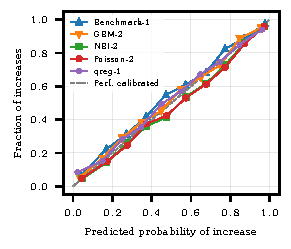
\includegraphics{plots/ed_arrival/60_reliability_diagram_lag_3}
    \caption{Reliability diagram for horizon three days.}\label{fig:app-eda-prob-rel-3}
    \end{subfigure}\hspace{0.01\textwidth}%
    \begin{subfigure}[t]{0.32\textwidth}
    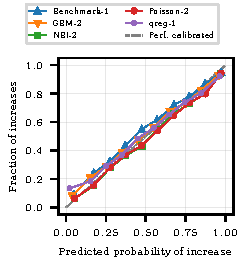
\includegraphics{plots/ed_arrival/60_reliability_diagram_lag_7}
    \caption{Reliability diagram for horizon seven days.}\label{fig:app-eda-prob-rel-7}
    \end{subfigure}
    \caption{Probabilistic trending evaluation for the models Benchmark-1, GBM-2, NBI-2, Poisson-2, and qreg-1 for the horizons three and seven days.}
    \label{fig:app-eda-prob}
\end{figure}

\subsubsection*{Discussion}

The trending ability is consistent for the two horizons, with the models' relative trending ability evolving similarly for the two horizons.
The models' trending ability is generally higher for the smaller horizon, but the differences are minor, and confidence intervals overlap.

The trending differs for all models for positive and negative predicted change directions.
While some models, such as GBM-2 and qreg-1, have the highest positive trending ratio, others, such as Poisson-2 and NBI-2, have the highest negative trending ratio.
Thus, the uncertainty of the model's predicted change has to be assessed differently based on the direction.

The results of the probabilistic trending evaluation endorse the point trending assessment and assign the best scores to NBI-2 and Poisson-2. 
The reliability diagrams show that they underestimate the fraction of increases slightly. 

The example shows that trending assessment is detached from standard point evaluation measures.
While the models with the lowest RMSE, NBI-2 and Poisson-2, also have a high trending ability, three models with below-average point evaluation measures, Benchmark-1, GBM-2, and qreg-1, have a high positive trending ability.


\subsection{Invasive and non-invasive blood pressure monitoring} \label{sec:application_measurement}

In the last briefer example, we consider the trending assessment of measurement data.
The data is from the MIMIC-III database, including various information on patients in critical care units of the Beth Israel Deaconess Medical Center in Boston (Massachusetts, USA, \cite{Johnson2016}).
The data is publicly available and also includes numerical measurement data such as heart rate, blood pressure, and oxygen saturation in a waveform database \citetext{\citealp{Moody2017}; available through \citealp{Goldberger2000}}.

For some patients, the data includes \ac{abp} and \ac{nbp} measurements.
While non-invasive blood pressure measurement methods are relatively gentle, they are less accurate than invasive methods.
For an overview of blood pressure measurement methods, see \citet{Saugel2014}.
For critical patients, changes in blood pressure can be crucial for the treatment.
Thus, trending assessment can be performed in addition to standard accuracy analysis~\citep[see, for example, ][]{Mostafa2020}.
Thus, we assess the trending ability of the non-invasive blood pressure measurements compared to the invasive blood pressure measurements.
The database contains 64,168 numerical data records.
One data record includes all numerical measurements for one patient.
The measured signals vary in length, frequency, and type of measurement.
Thus, only a subset of the data contains measurements of \ac{abp} and \ac{nbp} simultaneously.
2,548 include at least one measurement of systolic \ac{abp} and \ac{nbp} and 1,327 include at least one measurement of systolic \ac{abp} and \ac{nbp} at the same time; for the mean \ac{abp} and \ac{nbp}, the numbers are 2,605 and 1,516, respectively.

We consider the horizons of one minute, five minutes, and 15 minutes for the trending assessment, as those are typical intervals of NBP measurements.

\subsubsection*{Results}

Again, we exclude the smallest 10\% of absolute differences in trending assessment.
The resulting four-quadrant plots of the mean and systolic blood pressure measurements for the different horizons are shown in Figure~\ref{fig:app-mimic-4q}.
The number of points in the four-quadrant plot is smaller due to the restriction to data records with measurements of mean or systolic \ac{abp} and \ac{nbp} simultaneously for two consecutive times with the specified horizons.
Thus, we use the \ac{nbp} measurements as test method and the \ac{abp} measurements as gold standard.
For the systolic measurements, 290, 332, and 442 points are available for the horizons of one, five, and 15 minutes; for the mean measurements, 406, 430, and 542.

The trending ratios, including confidence intervals for the different horizons, are listed in Table~\ref{tab:app-mimic-trending-ratios}.
For the measurements with a horizon of one minute, the confidence intervals have lower bounds of 0.5 or slightly above.
For larger horizons, the trending ratio increases.
The difference between positive and negative trending ratios is small for all types and horizons, with overlapping confidence intervals.

Figure~\ref{fig:app-mimic-cond-prob} shows the conditional trending plots for the different horizons and the systolic and mean blood pressure measurements.
It becomes apparent that the systolic measurements have a higher trending ability than the mean measurement, except for small negative predicted changes.
This aligns with the trending ratios, but the confidence intervals overlap.

\begin{figure}
    \centering
    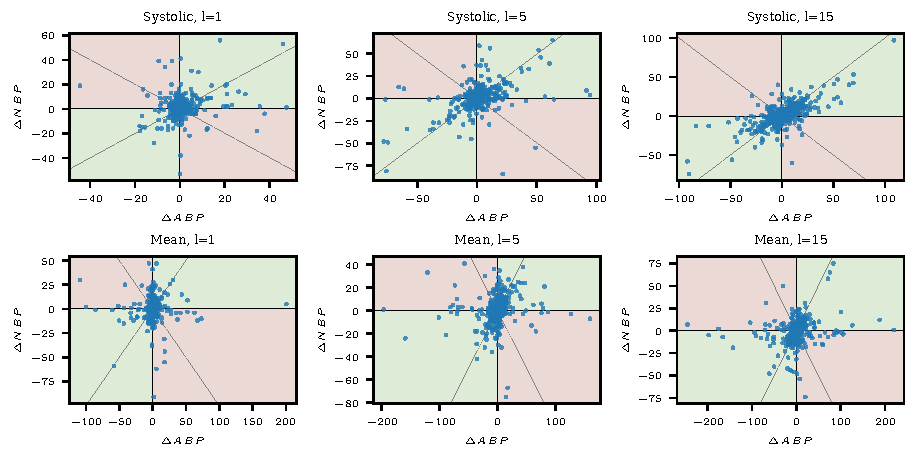
\includegraphics{plots/mimic/plot_4q}
    \caption{Four-quadrant plots for the different horizons and the systolic and mean blood pressure measurements. The upper row contains systolic measurements, and the lower row contains mean measurements. The columns contain the horizons one, five, and 15 minutes.}
    \label{fig:app-mimic-4q}
\end{figure}

\begin{table}
    \centering
    \begin{tabular}{l l p{0.2\textwidth} p{0.2\textwidth} p{0.2\textwidth}}
\toprule
Type & $l$ & $\mu^{l}$ & $\mu^{+, l}$ & $\mu^{-, l}$ \\
\midrule
Systolic & 1 & {0.55 (0.50, 0.60)} & {0.59 (0.52, 0.65)} & {0.58 (0.50, 0.66)} \\
Systolic & 5 & {0.63 (0.59, 0.68)} & {0.70 (0.64, 0.75)} & {0.62 (0.56, 0.69)} \\
Systolic & 15 & {0.69 (0.65, 0.73)} & {0.72 (0.66, 0.76)} & {0.74 (0.69, 0.79)} \\
Mean & 1 & {0.55 (0.51, 0.59)} & {0.62 (0.56, 0.68)} & {0.56 (0.50, 0.62)} \\
Mean & 5 & {0.59 (0.55, 0.64)} & {0.65 (0.59, 0.71)} & {0.62 (0.56, 0.68)} \\
Mean & 15 & {0.62 (0.58, 0.65)} & {0.65 (0.60, 0.70)} & {0.66 (0.61, 0.71)} \\
\bottomrule
\end{tabular}

    \caption{Trending ratios for the different horizons and the systolic and mean blood pressure measurements.}
    \label{tab:app-mimic-trending-ratios}
\end{table}

\begin{figure}
    \centering
    \begin{subfigure}[t]{.32\textwidth}
        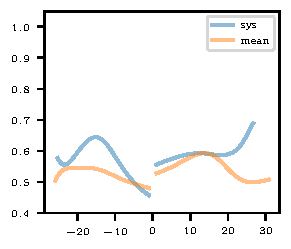
\includegraphics{plots/mimic/cond_prob_diff_nbp_abp_lag1}
        \caption{Horizon one minute.}
    \end{subfigure}\hspace{0.01\textwidth}
    \begin{subfigure}[t]{.32\textwidth}
        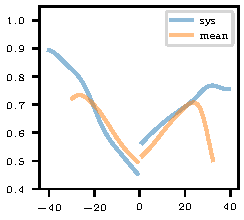
\includegraphics{plots/mimic/cond_prob_diff_nbp_abp_lag5}
        \caption{Horizon five minutes.}
    \end{subfigure}\hspace{0.01\textwidth}
    \begin{subfigure}[t]{.32\textwidth}
        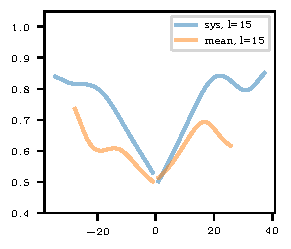
\includegraphics{plots/mimic/cond_prob_diff_nbp_abp_lag15}
        \caption{Horizon 15 minutes.}
    \end{subfigure}\hspace{0.01\textwidth}
    \caption{Conditional trending plot for the systolic and mean blood pressure measurements and the horizons one, five, and 15 minutes. }
    \label{fig:app-mimic-cond-prob}
\end{figure}




\subsubsection*{Discussion}

The four-quadrant plots contain a considerable number of extreme points.
Whether these points are due to measurement errors or extreme values is not distinguishable.
Some authors argue to exclude the measurements below the 10\%-quantile of the absolute differences and the points above the 90\%-quantile \citep[see][]{Critchley2010}.
We do not follow this approach here, as the extreme values are not necessarily measurement errors and could be particularly relevant.

The differences between positive and negative predicted changes are small in this example.
The positive and negative trending ratios have overlapping confidence intervals, and the conditional trending plots do not contain prominent deviations in the course.
This aligns with the four-quadrant plots, where no apparent asymmetry is visible.

The bootstrap confidence intervals are wide.
The width is around 0.1 for the trending ratio, while it gets up to 0.16 for the negative trending ratio for systolic measurement and the horizon of one minute.
Thus, more measurements would be of interest for a further trending assessment. 



\printbibliography

\appendix
\section{Data generation for Section~\ref{sec:trending}}\label{sec:app-trending-data-generation}
\section{Additional material on Section~\ref{sec:trending}}\label{sec:appendix-trending}

\subsection{Data generation for Section~\ref{sec:trending}}\label{subsec:app-trending-data-generation}

The first dataset is generated by sequentially generating $\diffx$ and $\diffy$.
First, the $\diffxt$ are sampled as a sum of a standard normal random number and a uniform random number on $(-10, 10)$:
\begin{equation*}
    \diffxt \sim N(0, 1) + U(-10, 10) \quad t = 1, \dots, T.
\end{equation*}
Subsequently, the $\diffy$ are simulated for a constant trending ratio $k$ by
\begin{equation*}
    \diffyt = \diffxt \cdot n_t \cdot b_t,
\end{equation*}
where $n_t$ is a truncated normal distribution with mean one and standard deviation 0.5, truncated at 0, and $b_t$ is a symmetric Bernoulli random variable with parameter $k$.
For a time-varying trending ratio, the parameter $k$ is modified to have a wave-shape over time, that is,
\begin{equation*}
    k_t = 0.75 + \sin(t / 365.25 \cdot 2 \pi) / 4.
\end{equation*}
For the asymmetric trending ratio, $k$ is a function of $\diffxt$,
\begin{equation*}
    k(x) = 0.5 + \min \left\{ \max \left\{ \frac{x + 5}{10}, 0  \right\} , 1 \right\} / 2.
\end{equation*}

In the second approach, $\diffyt$ and $\diffxt$ are modeled to be multivariate normal with mean 0 and covariance matrix
\begin{equation*}
    \Sigma = \begin{pmatrix} 4 & 3 \\ 3 & 4 \end{pmatrix}.
\end{equation*}
Thus, the conditional probability of trending can be calculated by a conditional normal distribution to
\begin{equation*}
    P(\diffyrv \diffxrv > 0 | \diffxrv = x) = \Phi \left( \frac{3}{2 \sqrt{7}} x \right),
\end{equation*}
where $\Phi$ is a standard normal \ac{cdf}.

The four-quadrant plots for the sample realizations of the data generation schemes are shown in Figure~\ref{fig:appendix_dgps}.

\begin{figure}
    \centering
    \begin{subfigure}{0.24\textwidth}
        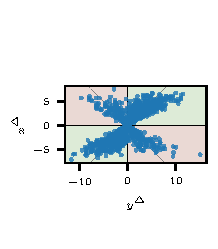
\includegraphics{plots/illustrative_examples/appendix_4q_dgp1}
        \caption{Constant trending ratio.}
    \end{subfigure}\hspace{0.01\textwidth}
    \begin{subfigure}{0.24\textwidth}
        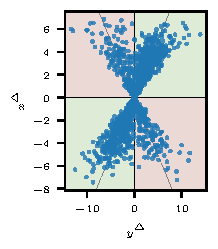
\includegraphics{plots/illustrative_examples/appendix_4q_dgp1_time}
        \caption{Time-varying trending ratio}
    \end{subfigure}\hspace{0.01\textwidth}
    \begin{subfigure}{0.24\textwidth}
        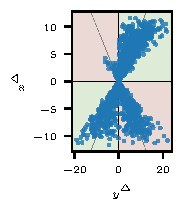
\includegraphics{plots/illustrative_examples/appendix_4q_dgp1_asym}
        \caption{Asymmetric trending ratio}
    \end{subfigure}\hspace{0.01\textwidth}
    \begin{subfigure}{0.24\textwidth}
        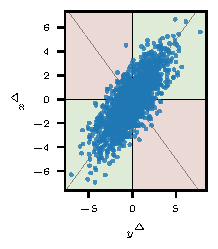
\includegraphics{plots/illustrative_examples/appendix_4q_dgp2}
        \caption{Second approach}
    \end{subfigure}
    \caption{Four-quadrant plots for sample realizations of the data generation schemes of Section~\ref{subsec:app-trending-data-generation}. Although the first and second plots differ over time, their difference is not discernible in the plots. The third data set's asymmetry is visible in the plot, but the decrease in the trending ability near 0 is not visible. }
    \label{fig:appendix_dgps}
\end{figure}

\subsection{Simulation study on bootstrapping confidence intervals}\label{subsec:appendix-trending-bootstrap}


We examine three methods for bootstrapping: the intuitive percentile and the more sophisticated basic and \ac{bca} method.
In the \textit{percentile} approach, the confidence interval for the level $\alpha$ is built directly from the empirical distribution of the bootstrap estimators.
The \textit{basic} approach computes the confidence interval based on the non-bootstrap estimate using the bootstrapped quantile deviations~\citep{Davison1997}.
The \ac{bca} method modifies the quantiles of the empirical bootstrap distribution by a bias and an acceleration parameter~\citep{Efron1987}.
Typically, the percentile approach needs larger datasets and provides an easy and fast estimate, while the \ac{bca} is computationally expensive but requires smaller datasets for reasonable confidence intervals.
The basic approach balances these two objectives.
We compare the approaches in a small synthetic data study on their small-dataset behavior and computation time.

We vary the number of available time steps $T$ to be a typical time-series value, such as 30 for daily data in a month, 52 for weekly data, 168, 365, 720, and 1024.
The considered datasets are the first dataset with asymmetric dependence and the second dataset outlined in Appendix~\ref{subsec:app-trending-data-generation}.
In the calculations, the \verb|scipy| package's implementation of bootstrap confidence intervals is used~\citep{Virtanen2020}.
The prescribed confidence level is 90 \%, and the number of bootstrap samples is $10,000$.
The share of confidence intervals covering the true values per method and $T$ are shown in Table~\ref{tab:trending_bootstrap}.
The true values of the accuracy are computed based on a dataset of size $10^8$, yielding 0.7501 and 0.7700 for the two datasets.
The computation times per method and dataset are shown in Figure~\ref{fig:trending_bootstrap_time}.
For the small sample sizes up to $T = 168$, only the \ac{bca} method keeps the confidence interval size and yields slightly wider confidence intervals.
The method's results do not differ for the larger sample sizes.
The computation time for the \ac{bca} method is slightly larger than for the other methods, but all methods have a moderate computation time.
\Ac{bca} is the only method that maintains the confidence level for small datasets while increasing the computation time only moderately for larger datasets.
Therefore, we use the \ac{bca} method for confidence intervals in the applications in Section~\ref{sec:application}.


\begin{table}
    \centering
    \tiny
    \begin{subtable}{.48\textwidth}
        \begin{tabular}{llll}
\toprule
 & percentile & basic & bca \\
\midrule
30 & 0.84 (0.249) & 0.86 (0.250) & 0.91 (nan) \\
52 & 0.89 (0.194) & 0.89 (0.193) & 0.89 (0.198) \\
168 & 0.91 (0.109) & 0.90 (0.109) & 0.90 (0.110) \\
365 & 0.90 (0.074) & 0.90 (0.074) & 0.90 (0.074) \\
720 & 0.90 (0.053) & 0.90 (0.053) & 0.90 (0.053) \\
1024 & 0.90 (0.044) & 0.90 (0.044) & 0.89 (0.044) \\
\bottomrule
\end{tabular}

        \caption{First dataset}
    \end{subtable}\hspace{0.02\textwidth}
    \begin{subtable}{.48\textwidth}
        \begin{tabular}{llll}
\toprule
 & percentile & basic & BCa \\
\midrule
30 & 0.87 (0.243) & 0.88 (0.242) & 0.92 (0.249) \\
52 & 0.87 (0.188) & 0.89 (0.188) & 0.90 (0.192) \\
168 & 0.89 (0.106) & 0.90 (0.106) & 0.90 (0.107) \\
365 & 0.90 (0.072) & 0.90 (0.072) & 0.90 (0.072) \\
720 & 0.90 (0.052) & 0.90 (0.052) & 0.90 (0.052) \\
1024 & 0.89 (0.043) & 0.90 (0.043) & 0.90 (0.043) \\
\bottomrule
\end{tabular}

        \caption{Second dataset}
    \end{subtable}
    \caption{Proportion of bootstrapping confidence intervals covering the true value of trending ratio per method and sample size $T$. The average width of the confidence interval is listed in brackets.}
    \label{tab:trending_bootstrap}
\end{table}

\begin{figure}
    \centering
    \begin{subfigure}{0.48\textwidth}
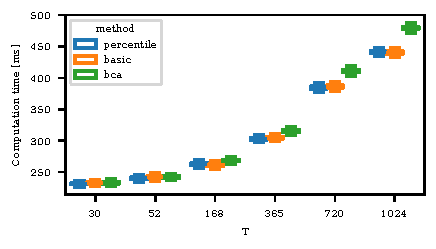
\includegraphics{plots/illustrative_examples/boxplot_comp_time_butterfly}
        \caption{First dataset}
    \end{subfigure}
    \begin{subfigure}{0.48\textwidth}
    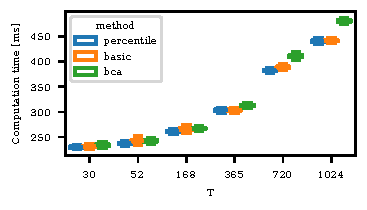
\includegraphics{plots/illustrative_examples/boxplot_comp_time_normal}
        \caption{Second dataset}
    \end{subfigure}
    \caption{Boxplot of the computation time of the different bootstrapping method and data set sizes $T$. The computation time refers to bootstrapping one confidence interval based upon $10,000$ values. Each boxplot reflects $10,000$ samples. The \ac{bca} method takes slightly longer than the other two, but the difference is negligible.}
    \label{fig:trending_bootstrap_time}
\end{figure}


\subsection{Visualization of different bandwidth selectors in multivariate \ac{kde}}\label{subsec:appendix-kde}

We examine the resulting conditional trending plots for the three well-known selectors, rule-of-thumb, cross-validation maximum likelihood, and cross-validation least squares using the \verb|statsmodels| Python package~\citep{Seabold2010} in Figure~\ref{fig:trending-cond-prob-bw}.
While the rule-of-thumb is based only on the covariance matrix, the other two numerically optimize the bandwidth with a hold-one-out least squares or likelihood objective function.
The dashed line shows the theoretical $P(\diffyrv \diffxrv > 0 | \diffxrv = x)$.
The second method, cross-validation least squares, requires long computation times while yielding small or no bandwidth results, even for two relatively small datasets.
The rule-of-thumb and cross-validation maximum likelihood methods yield reasonable results at moderate computation times. 
Further examples, including comparisons between methods regarding their trending ability, are available in Section~\ref{sec:application}.

\begin{figure}
    \centering
    \begin{subfigure}{.48\textwidth}
        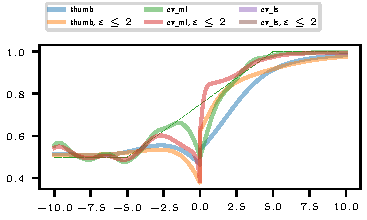
\includegraphics{plots/illustrative_examples/cond_prob_plot_bw_butterfly}
        \caption{First dataset with asymmetric dependence.}
    \end{subfigure}
    \begin{subfigure}{.48\textwidth}
        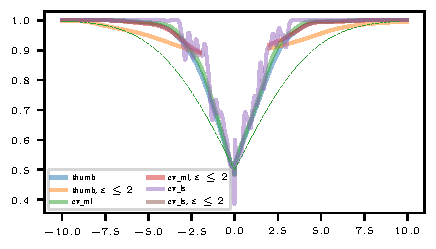
\includegraphics{plots/illustrative_examples/cond_prob_plot_bw_normal}
        \caption{Second dataset. }
    \end{subfigure}
    \caption{Resulting conditional trending plot for different bandwidth selection processes. Cross-validation least squares takes a considerably larger computation time. It does not converge for the first data set and yields a bandwidth too small for the second data set. The rule of thumb is the fastest method but tends to oversmooth. The cross-validation maximum likelihood method yields a more reasonable bandwidth with moderate computation time. $\varepsilon$ specifies an exclusion area $E = \{(x, y) \in \R^2: (-\varepsilon \leq x \leq \varepsilon)\}$ in $\diffx$-direction.}\label{fig:trending-cond-prob-bw}
\end{figure}




\subsection{Probabilistic trending evaluation}

If forecasts or nowcasts are given as quantiles, $p_t$ can be determined by interpolations among the quantiles.
Let $q_p$ denote the quantiles for forecast time $t+l$ for even-spaced probabilities $p \in \{1/\pmax, \dots, (p-1) / \pmax\}$ ($\pmax \in \N \setminus \{1, 2\}$) and $y_t$ the true value at time $t$.
The quantiles $q_p$ generally differ for each time step, but we omit an index here for ease of notation.
The probability $\pc_t$ of a \textit{negative} change is between $p^{\star}$ and $p^{\star} + 1/\pmax$ for
\begin{equation*}
    p^{\star} = \max \{p \in \{1/\pmax, \dots, (\pmax-1) / \pmax\}: q_p \leq y_t\} , \quad \text{if}\ q_{1/\pmax} \leq y_t \leq q_{1 - 1/\pmax}.
\end{equation*}
Quantiles do not determine the location within the interval $[p^{\star}, p^{\star} + 1/\pmax]$.
Under the assumption of a uniform distribution within the quantile interval, the probability of a negative change is
\begin{equation*}
    \pc_t = \frac{y_t - q_{p^\star}}{\pmax (q_{p^{\star} + 1} - q_{p^{\star}})} + p^{\star}.
\end{equation*}
The approach does not assign probabilities for $y_t$ smaller than the smallest quantile $q_{1/p}$ or larger than the largest quantile.
As a simple extension, we assume that the probability mass is uniformly distributed on an interval of the same length as the nearest interval specified by the quantiles.
This yields
\begin{equation*}
\pc_t = \begin{cases}
    \max \{\frac{1}{\pmax} - \frac{q_{p^\star} - y_t}{\pmax (q_{p2/\pmax} - q_{1/\pmax})}, 0\} &, \text{if } y_t < q_{1/p}, \\
    \min \{\frac{1}{\pmax} - \frac{y_t - q_{(\pmax-1)/\pmax}}{\pmax (q_{(\pmax-1)/\pmax} - q_{(\pmax-2)/\pmax})}, 1\} &, \text{if } y_t > q_{1 - 1/p}, \\
    \frac{y_t - q_{p^\star}}{\pmax (q_{p^{\star} + 1} - q_{p^{\star}})} + p^{\star} &, \text{otherwise.}
\end{cases}
\end{equation*}
The probability of positive change is $p_t = 1 - \pc_t$.

If the true value is given as a distribution because it is still unknown, the probabilities $p_t$ can be computed by integration.
Let for two nowcasts the distributions be given by \acp{pdf} $f_{t+l|t+l}$ and $f_{t|t+l}$ with \acp{cdf}  $F_{t+l|t+l}$ and $F_{t|t+l}$.
Then, the probability of a negative change can be computed by
\begin{align}
    \pc_t
        &= \int_{\begin{subarray}{l}x_1, x_2 \in \R: \\ x_2 < x_1\end{subarray}} f_{t|t+l} (x_1) f_{t+l|t+l} (x_2)  \ \textrm{d} \: (x_1, x_2) \nonumber\\
        &= \int_{x_1 \in \R} \int_{-\infty}^{x_1} f_{t|t+l} (x_1) f_{t+l|t+l} (x_2)  \ \textrm{d} \: x_2 \ \textrm{d} \: x_1 \nonumber\\
        &= \int_{x_1 \in \R} f_{t|t+l} (x_1) F_{t+l|t+l} (x_1)  \ \textrm{d} \: x_2 \ \textrm{d} \: x_1 \label{eq:trending-probabilistic-pdf}.
\end{align}
Thereby, the distributions are assumed to be independent.
If the nowcasts have the form of a multivariate distribution, including the dependence of the two \acp{pdf}, $f_{t+l|t+l} (x_2)$ has to be replaced by the \ac{pdf} conditional on $x_1$.
As a Monte Carlo approximation of Equation~\eqref{eq:trending-probabilistic-pdf}, the probability can also be calculated by sampling from $f_{t+l|t+l}$ and $f_{t|t+l}$ and calculating the fraction of negative changes.
For forecasts, the indexes have to be shifted.
If no \acp{pdf} are available, they can be estimated from the \ac{cdf} or quantiles, or the \ac{cdf} or quantiles can be used to generate samples for the Monte Carlo approximation.






\end{document} 